\chapter{Resultados de Comportamientos emergentes en Robots con el  Conectoma de C. elegans}\label{cap:resultados_robot}
\graphicspath{{figs/capitulo_resultados_robot/}}

\chapterquote{Far from being able to accept the idea of the individuality and independence of  	each nerve element, I have never had reason, up to now, to give up the concept 	which I have always stressed, that nerve cells, instead of working individually, act 	together [...]. However opposed it may seem to the popular tendency to individualize the elements, I cannot abandon the idea of a unitary action of the 	nervous system [...]}{Camillo Golgi, 1906}


El comportamiento adaptativo es un atributo distintivo de los organismos vivos y se manifiesta en su capacidad para responder con flexibilidad a las señales sensoriales. La comprensión de cómo los circuitos neuronales logran esta adaptabilidad es esencial para la neurociencia y la inteligencia artificial. En particular, es crucial descubrir cómo un conectoma anatómicamente estático puede ser modulado para permitir la regulación dinámica de la conectividad funcional en la red neuronal. En esta sección, mostraremos los resultados de  una investigación que se embarcó en el desafío de abordar esta cuestión fundamental.

La orientación en el entorno es una habilidad fundamental para un robot autónomo. En la naturaleza, los seres vivos, incluso los más simples, exhiben impresionantes capacidades de control de orientación. La supervivencia de muchas especies depende en gran medida de su capacidad para navegar en el espacio, lo que les permite buscar refugio, encontrar recursos alimenticios y emparejarse. Los mecanismos que permiten a los organismos detectar y responder a una amplia variedad de estímulos ambientales han evolucionado a lo largo del tiempo. Esta capacidad de orientación se ha convertido en un enigma intrigante y un punto de partida inspirador para el diseño de controladores de orientación de robots.

La importancia de comprender los mecanismos de control motor no puede subestimarse. Por lo tanto, en esta investigación, utilizamos un robot que incorpora el conectoma de C. elegans, un organismo modelo ampliamente estudiado en la biología. Nuestra elección se basa en la idea de que la eficacia de un robot en tareas de navegación y evitación de obstáculos podría arrojar luz sobre el funcionamiento de la habilidad motora de un organismo vivo. Para evaluar esta eficacia, diseñamos y ejecutamos una serie de experimentos en un entorno altamente controlado. Nuestro enfoque no se limita a un solo robot, sino que involucra tanto al robot comercial GoPiGo como a un robot de construcción personalizada. Esta elección meticulosa garantiza que los resultados sean consistentes y reproducibles en diferentes configuraciones y con diversas plataformas de robots.

El resultado de nuestros experimentos demostró la capacidad de los robots para detectar obstáculos y ajustar sus trayectorias, lo que a su vez les permitió navegar de manera segura en su entorno. Estos resultados son prometedores y abren la puerta a nuevas perspectivas para el diseño de robots autónomos y la comprensión de los principios subyacentes a la orientación en el espacio.

Este capítulo presenta los resultados de nuestra investigación y ofrece una visión más profunda de la relación entre el conectoma, la función y el comportamiento. Nuestros experimentos tienen como objetivo desentrañar cómo se ensamblan las dinámicas de la red neuronal y cómo la estructura del conectoma y las conexiones sinápticas dan lugar a los comportamientos observados. Además, buscamos identificar en la dinámica de los robots algunas características fundamentales que pueden compararse con la dinámica neuronal global de C. elegans. Al explorar la presencia de grupos de neuronas sincronizadas y una estructura jerárquica anidada, buscamos establecer vínculos entre la compleja estructura de red del connectoma y las características emergentes en la dinámica del robot.

Estos resultados no solo tienen implicaciones para la comprensión de cómo los organismos vivos se adaptan y responden a entornos cambiantes, sino que también abren nuevas vías de investigación en el campo de la inteligencia artificial. Al dotar a sistemas cibernéticos con características complejas inspiradas en seres vivos, podríamos avanzar hacia una nueva generación de inteligencia artificial que se base en principios biológicos. Además, la capacidad de realizar experimentos controlados con un organismo cibernético nos permitirá probar hipótesis de manera precisa y avanzar en nuestra comprensión de la adaptación biológica.

Esta sección de resultados es un paso importante hacia la confluencia de la biología y la robótica, y esperamos que los hallazgos presentados aquí inspiren investigaciones futuras en campos interdisciplinarios y abran nuevas perspectivas sobre la adaptación y la inteligencia.

 
\section{Evaluación del Comportamiento del Neurorobot}

Antes de llevar a cabo cualquier medición o análisis de la dinámica neuronal simulada del C. elegans, así como del comportamiento emergente del neurorobot en el que se implementa, es esencial garantizar la robustez y la idoneidad de los parámetros que controlan la dinámica neuronal del modelo. Además, se debe asegurar que el comportamiento resultante sea coherente con lo observado en organismos reales. En esta sección, se llevaron a cabo un conjunto de pruebas para verificar el óptimo funcionamiento de los algoritmos que simulan la dinámica neuronal del C. elegans y el comportamiento que emerge del robot.

\subsection{Prueba del Parámetro de Umbral ($h$)}	

La dinámica microscópica de nuestro modelo neurorobótico, expresada en la ecuación 1, se encuentra bajo la influencia de un parámetro de control denominado $h$. Con el fin de examinar cómo varía el comportamiento emergente en función de este parámetro, se llevaron a cabo experimentos de cinco minutos en varios rangos de valores de $h$. Posteriormente, se analizaron tanto el comportamiento macroscópico del robot como las matrices de dinámica neuronal y de acciones registradas. Los resultados se presentan en las \Cref{fig:valores_neuronas_umbrales,fig:accion_umbrales} .


\begin{figure}[h!]
	\centering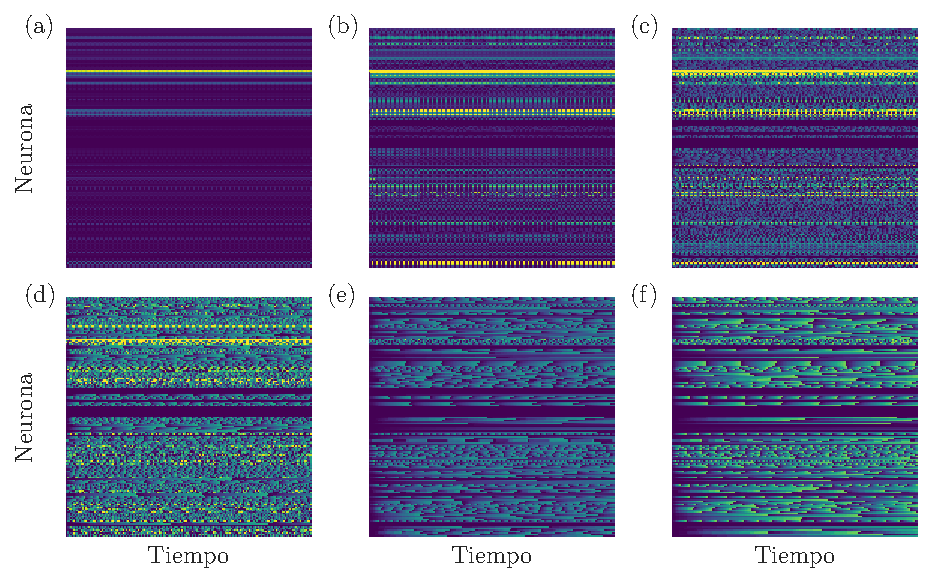
\includegraphics[width=\imsize]{valores-neuronas_umbrales.pdf}
	\caption[ Resultados de la Prueba del Parámetro de Umbral ($h$).]{ Las subfiguras (a-b) muestran la actividad de las neuronas cuando el umbral $h$ es demasiado bajo, lo que conduce a un comportamiento tipo epileptoide. En las subfiguras (c-d), se observa que la actividad neuronal se apaga cuando el umbral es demasiado alto, resultando en un estado comatoso del robot. Finalmente, en las subfiguras (e-f), se muestra la actividad óptima con un umbral intermedio, similar a los experimentos con organismos reales. }\label{fig:valores_neuronas_umbrales}
\end{figure}


\begin{figure}[h!]
	\centering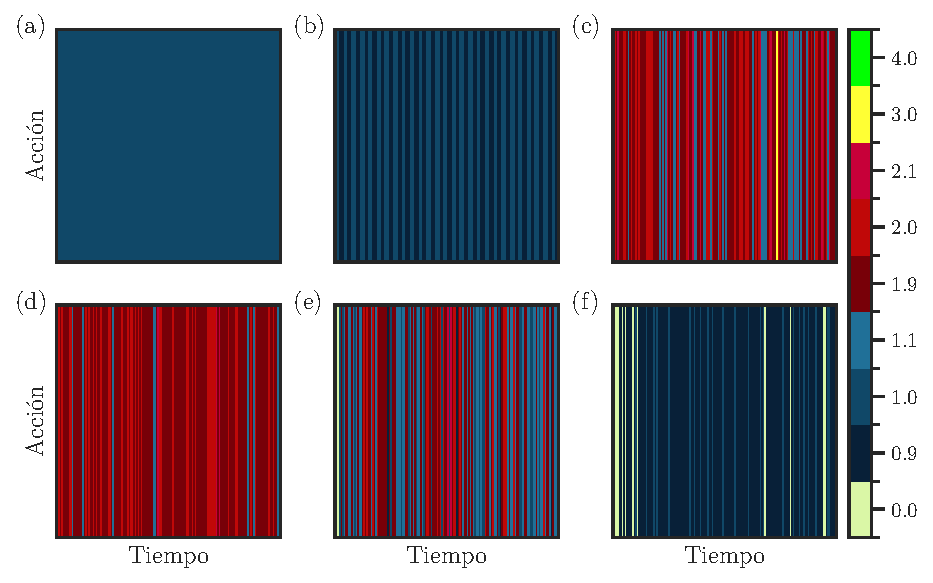
\includegraphics[width=\imsize]{accion_umbrales.pdf}
	\caption[ Matrices de Acciones Correspondientes a la Prueba de Umbral ($h$).]{ Matrices de Acciones Correspondientes a la Prueba de Umbral ($h$). Las subfiguras (a-b) muestran las acciones del robot cuando el umbral $h$ es demasiado bajo, lo que resulta en un comportamiento caótico. En las subfiguras (c-d), se observa la ausencia de movimiento cuando el umbral es demasiado alto. Por último, en las subfiguras (e-f), se representan las acciones complejas y coherentes con un comportamiento emergente óptimo, como el retroceso al encontrar obstáculos, cuando se utiliza un umbral intermedio. }\label{fig:accion_umbrales}
\end{figure}





Cuando el umbral $h$ es demasiado bajo (por ejemplo, $h=1$ o $h=5$), la mayoría de las neuronas disparan en cada paso de tiempo (\Cref{fig:valores_neuronas_umbrales}a-b). Este fenómeno resulta en la ausencia de una actividad de red rica y coordinada, es decir, no se observan grupos de neuronas sincronizadas. Como consecuencia, el comportamiento del robot se asemeja a un estado epiléptico, con giros en múltiples direcciones y avance constante, como se refleja en la matriz de acciones registrada (\Cref{fig:accion_umbrales}a-b). En estos valores, no se manifiestan comportamientos emergentes significativos.

Por otro lado, cuando el umbral es demasiado alto ($h>100$), casi ninguna neurona dispara, ya que se requieren numerosos pasos de tiempo para que las neuronas alcancen el umbral. En este escenario, la actividad de la red neuronal se encuentra apagada (\Cref{fig:valores_neuronas_umbrales}c-d), con un número reducido de neuronas sincronizadas. Esto conduce a un comportamiento que se asemeja a un estado comatoso del robot, donde prácticamente no se observa movimiento (\Cref{fig:accion_umbrales}c-d).

Finalmente, se observa que solo en los rangos intermedios (por ejemplo, $h=15$ y $h=30$), la actividad de la red muestra grupos de neuronas sincronizadas (\Cref{fig:valores_neuronas_umbrales}e-f), similar a lo que se observa en experimentos con organismos reales. Las matrices de acciones (\Cref{fig:accion_umbrales}e-f) concuerdan con un comportamiento emergente que implica acciones complejas, como la capacidad de retroceder al encontrar un obstáculo. Por lo tanto, se concluye que el comportamiento emergente del robot es óptimo en los rangos intermedios del umbral. Es importante destacar que, no obstante, este valor no requiere un ajuste preciso, ya que se obtuvieron resultados cualitativamente similares para umbrales que oscilan entre 10 y 100. Basándonos en estos resultados, se optó por el valor de umbral de 30 para el resto de los experimentos.

\subsubsection{Discusión}

Los hallazgos anteriores sugieren un comportamiento crítico, similar a lo que se observa en la física estadística de las transiciones de fase. En este contexto, los comportamientos más complejos se manifiestan únicamente en una región de este diagrama, que se denomina \textquote{región crítica}. Estos resultados sugieren que el sistema nervioso de los organismos podría manifestar su óptimo funcionamiento dentro de un rango crítico. Motivados por estos hallazgos, en la segunda parte de esta tesis se profundiza en la hipótesis anteriormente mencionada, conocida en la literatura como la \textquote{hipótesis de criticidad neuronal}.

\subsection{Variación de las Pausas y su Impacto en el Comportamiento}

La observación del comportamiento emergente en el neurorobot plantea una interrogante fundamental: ¿Cómo es posible que una red neuronal, adaptada para controlar la locomoción de un gusano de apenas 1 mm de longitud, pueda aplicarse de manera efectiva en el control de un vehículo robótico de aproximadamente 30 cm de longitud? Esta sección muestra los resultados de investigar en profundidad cómo la incorporación estratégica de pausas en el programa de control, con una variación de duraciones que oscila entre 0.5 y 0.8 segundos, permite al robot ejecutar con precisión los comandos transmitidos por el conectoma. Este enfoque se traduce en una sincronización exitosa entre la escala temporal de las simulaciones y la escala de respuesta del vehículo robótico, lo que plantea la posibilidad de aplicar el conectoma del C. elegans para controlar robots de distintos tamaños. Esta sección se centra en el análisis de cómo la variación de las pausas afecta el comportamiento del robot.

Para alcanzar este objetivo, se llevaron a cabo experimentos de un minuto de duración, en los cuales se empleó el neurorobot para simular la dinámica neuronal del C. elegans con diferentes valores de pausas entre la emisión de comandos y la ejecución de acciones. El análisis se centró en la relación entre los comandos enviados al robot y las acciones efectivamente realizadas. Se encontró la  existencia de un amplio rango de duraciones de pausas en el que el robot exhibe un comportamiento similar. Sin embargo, se observa que cuando las pausas son notoriamente cortas, el robot no puede seguir las acciones con la suficiente velocidad, lo que da lugar a un comportamiento errático que, en última instancia, paraliza el movimiento del robot. El análisis de las matrices de acciones revela que muchas de las acciones programadas superan las limitaciones de velocidad del robot, lo que resulta en la no ejecución de más de la mitad de las acciones planificadas. Por otro lado, cuando las pausas son significativamente prolongadas, el robot experimenta considerables retrasos en la ejecución de acciones. En estas condiciones, las matrices de acciones exhiben intervalos extensos entre las acciones, semejantes a las de un organismo con un metabolismo considerablemente lento. Solo en valores intermedios de la duración de las pausas se consigue un comportamiento adecuado que permite la ejecución de acciones sin que se superpongan.

Las \Cref{fig:pause_bajo,fig:pause_alto} presentan una representación gráfica de las matrices de acciones correspondientes a pausas de duración corta y larga, respectivamente. En la Figura 1, se observa una alta densidad de acciones programadas en un espacio de tiempo breve, lo que sobrecarga al robot y produce un comportamiento caótico. Por otro lado, en la Figura 2, la escasa densidad de acciones indica una larga duración entre cada acción



\begin{figure}[h!]
	\centering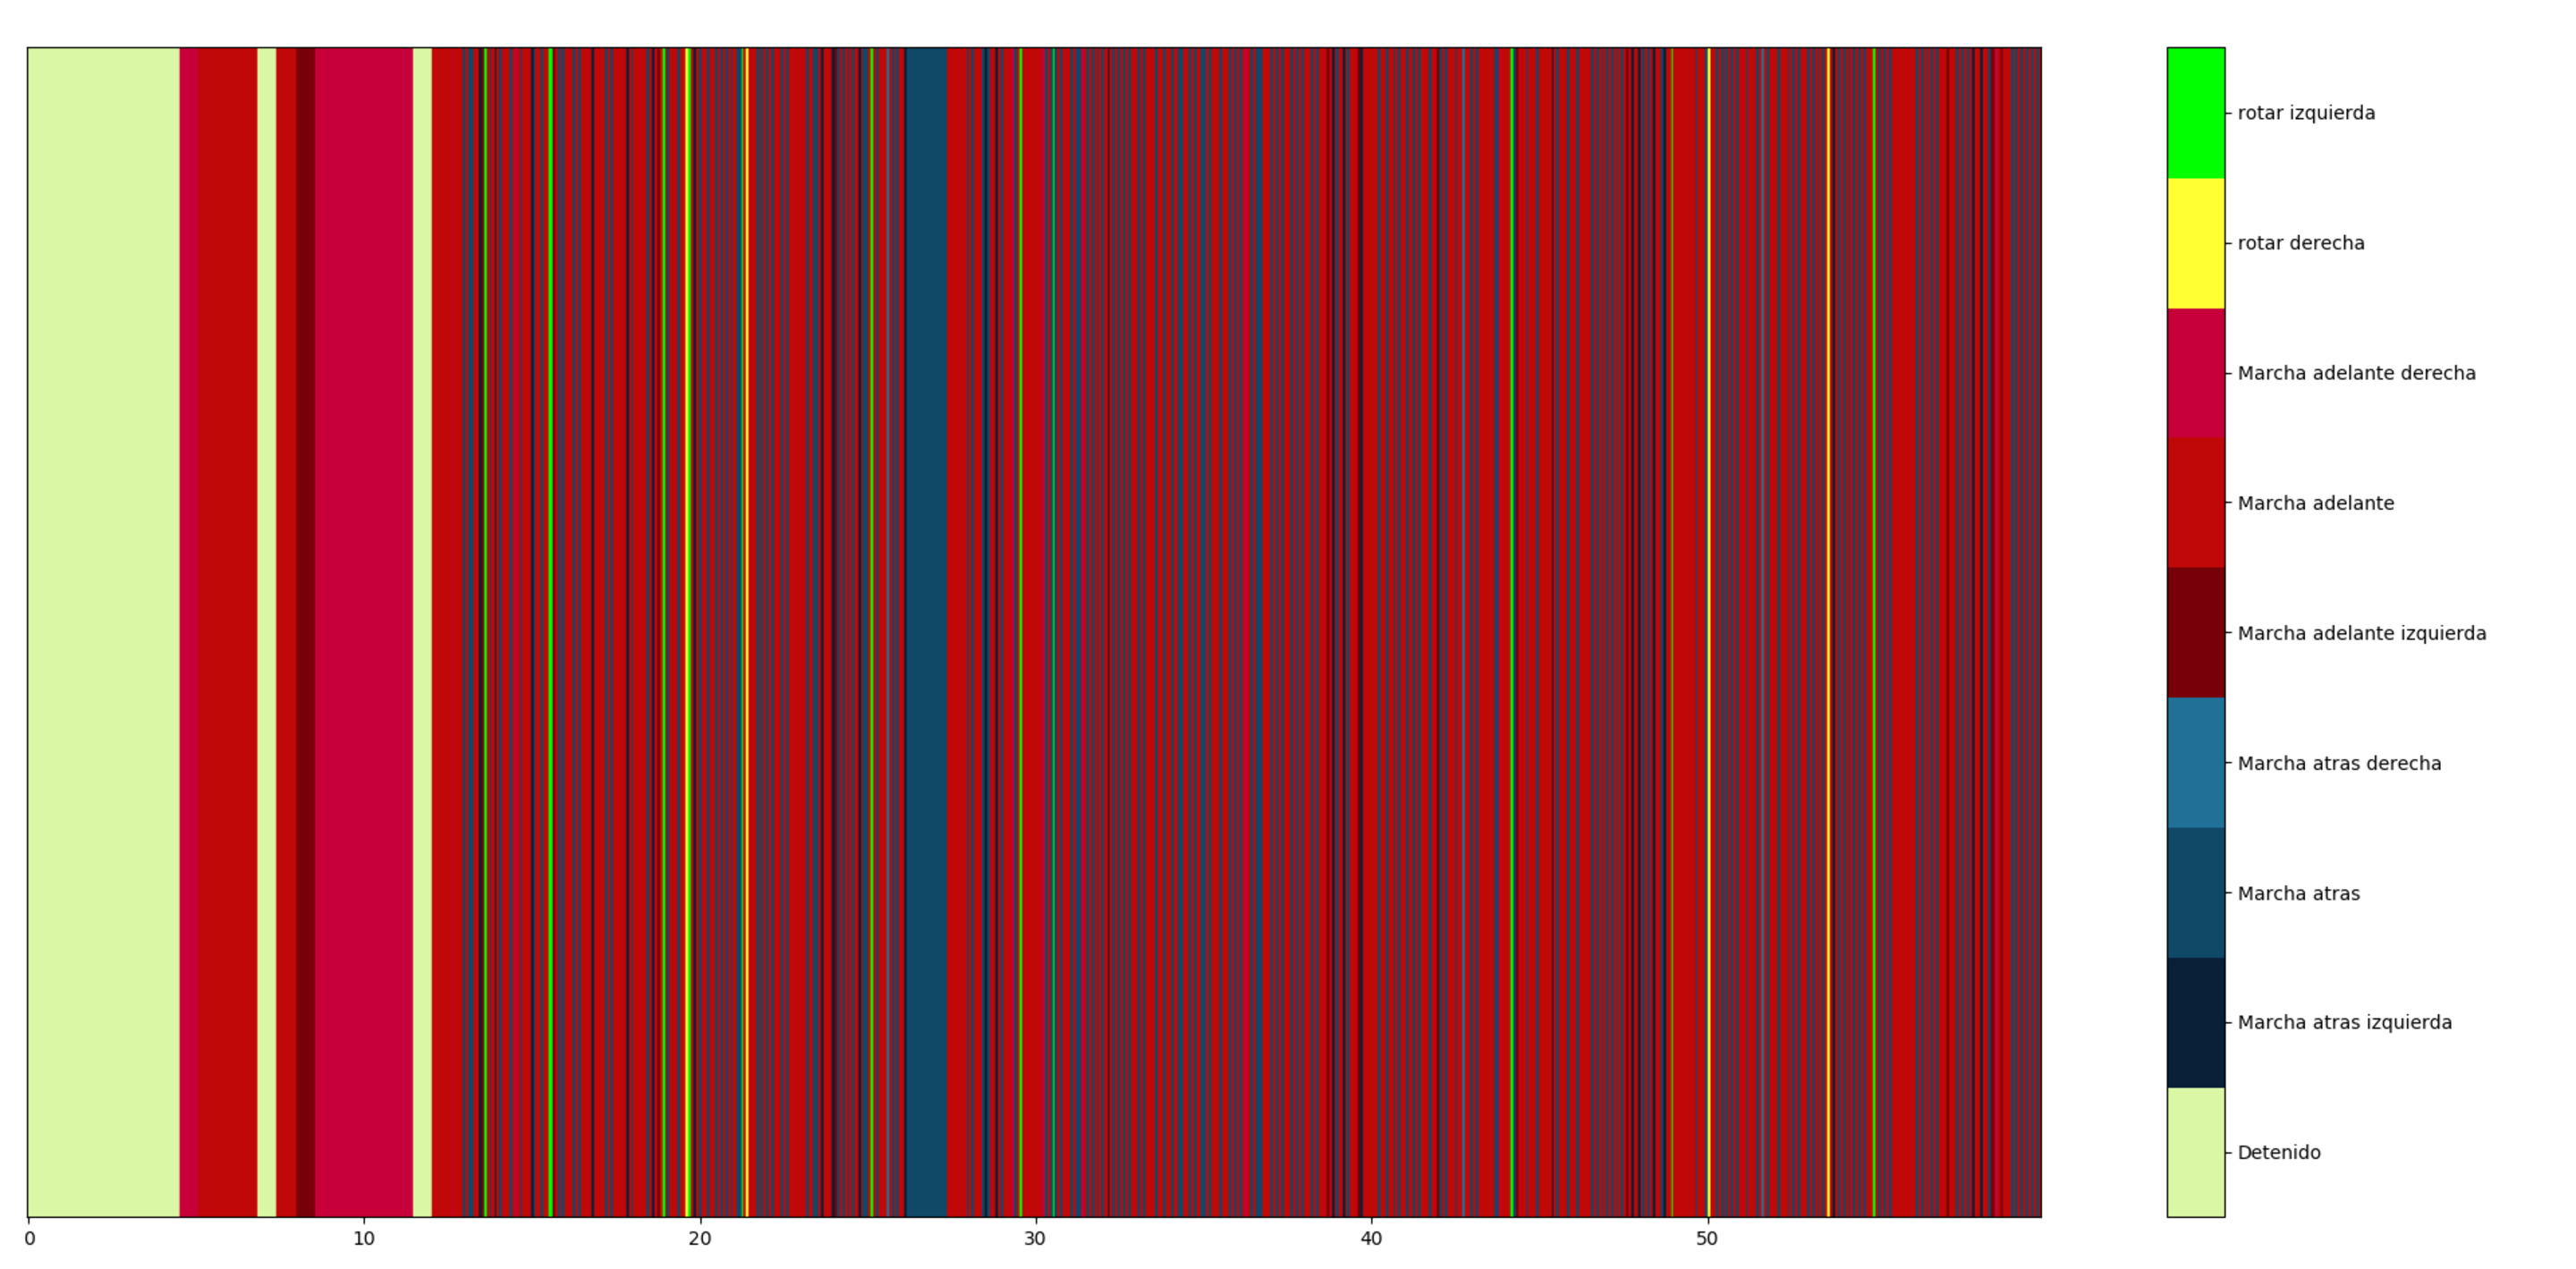
\includegraphics[width=\imsize]{pause_bajo.pdf}
	\caption[ Matriz de Acciones con Pausas largas.]{ Matriz de Acciones con Pausas largas. Esta figura presenta una matriz de acciones generada durante experimentos con pausas largas en el programa de control del robot, lo que da como resultado una baja densidad de acciones y un comportamiento más lento y deliberado, similar al de un organismo con un metabolismo lento.}\label{fig:pause_bajo}
\end{figure}


\begin{figure}[h!]
	\centering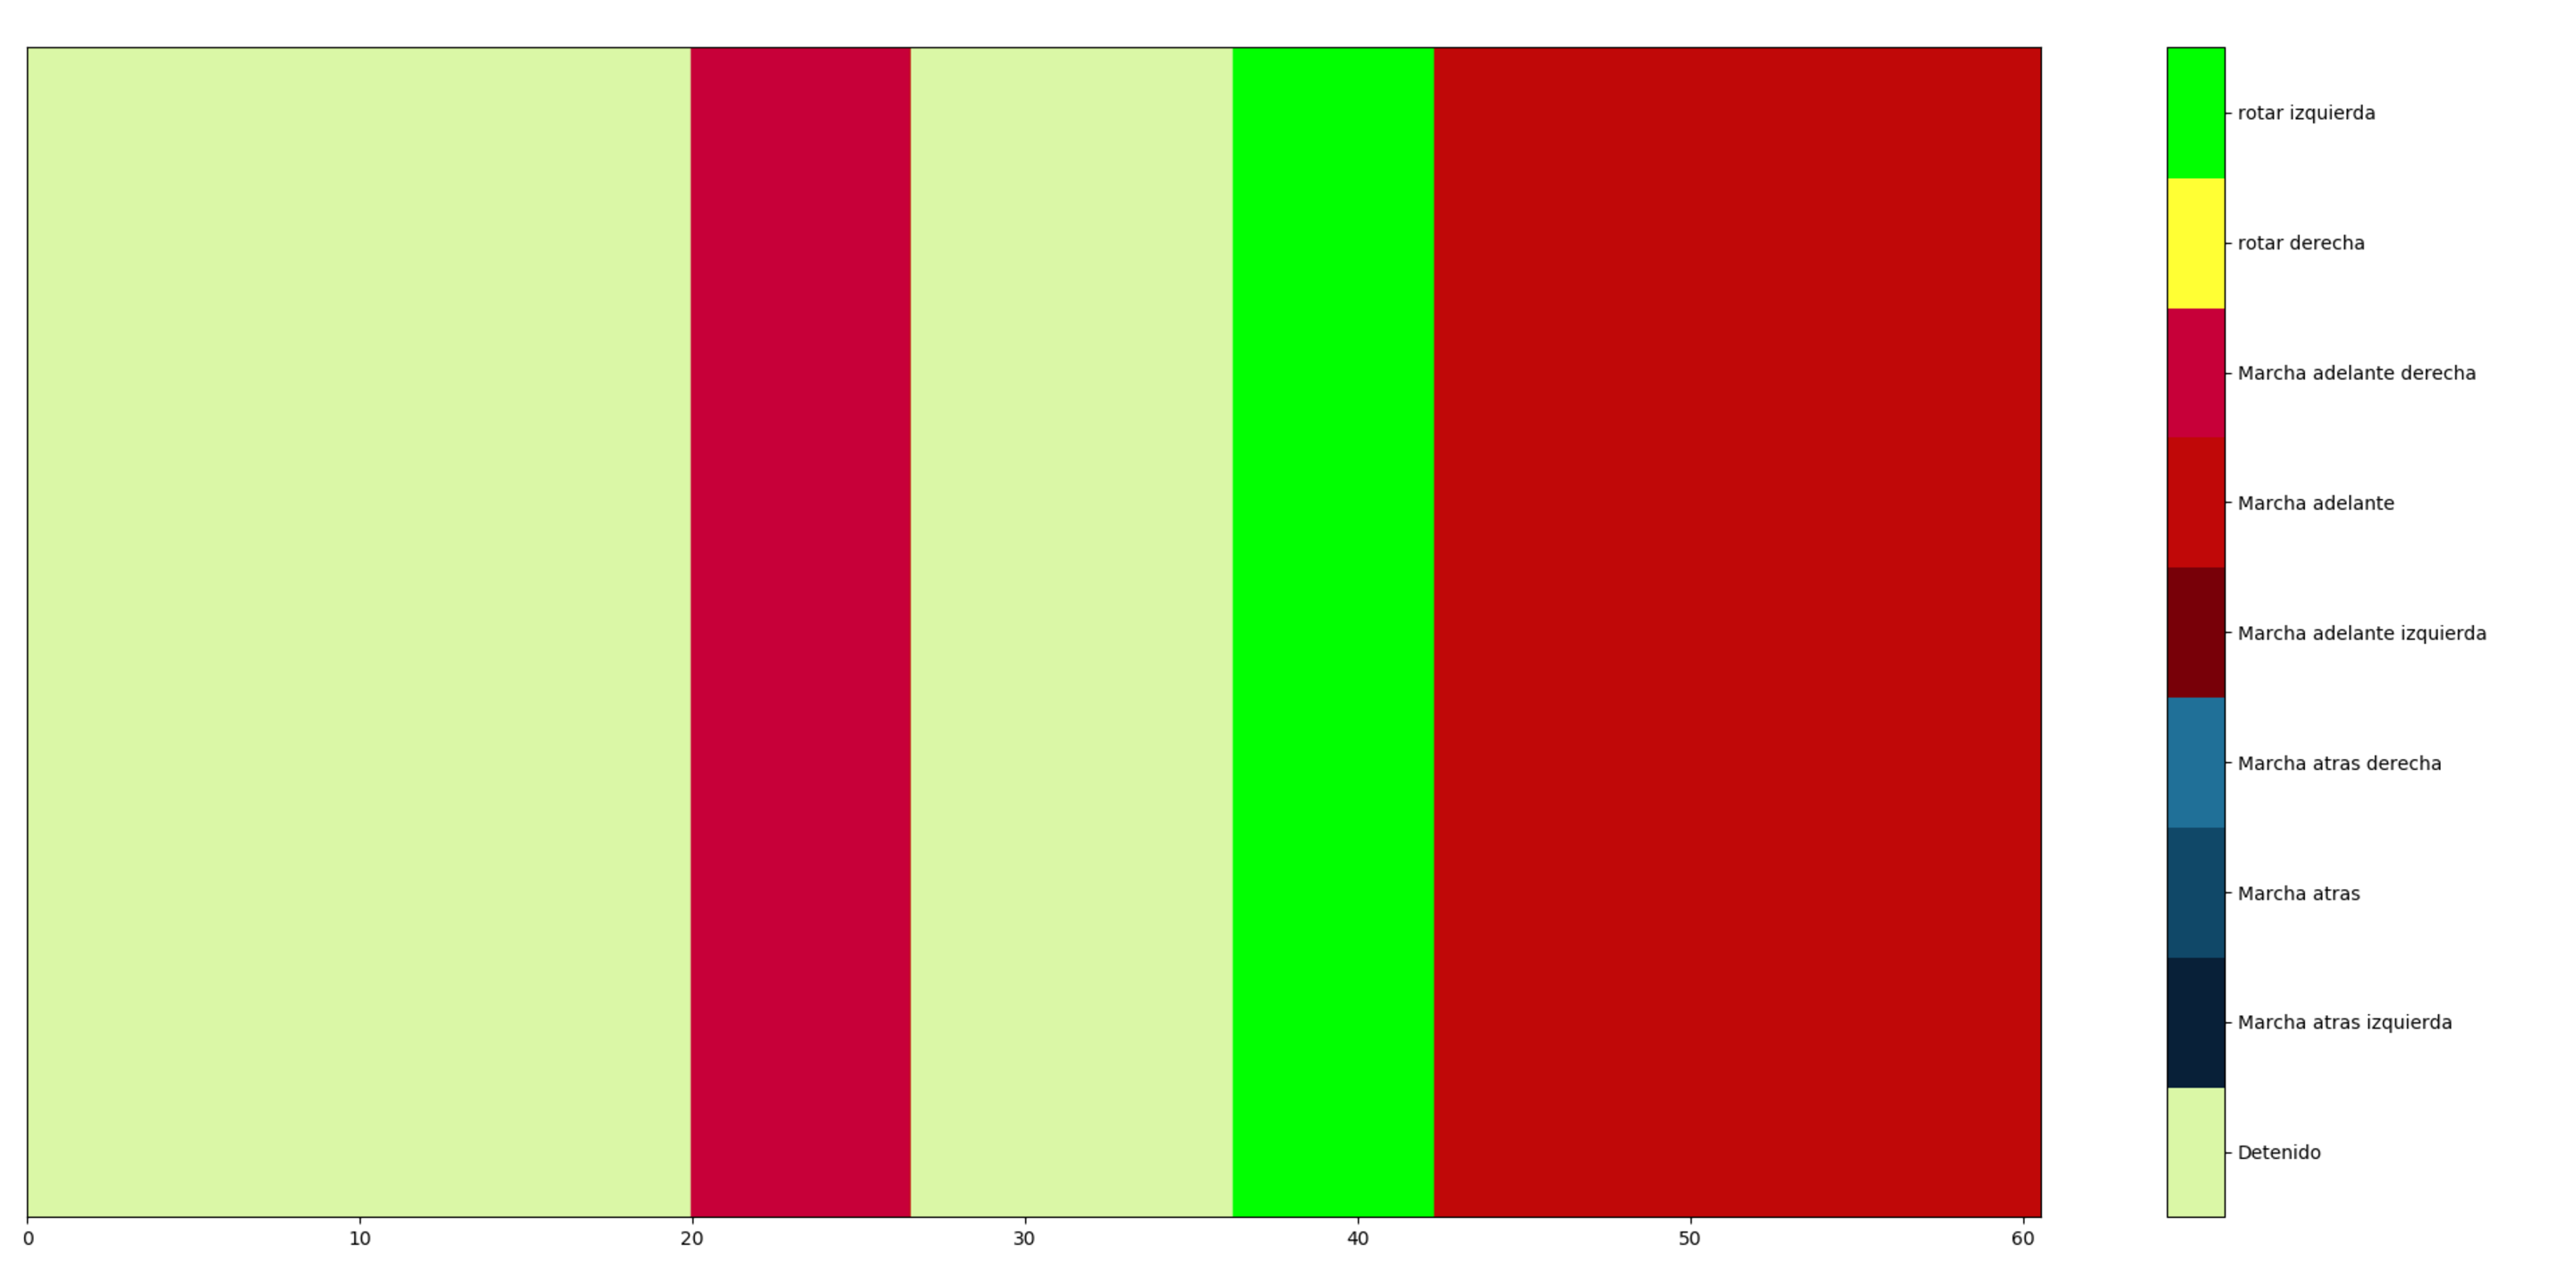
\includegraphics[width=\imsize]{pause_alto.pdf}
	\caption[ Matriz de Acciones con Pausas Cortas.]{ Matriz de Acciones con Pausas Cortas. Esta figura ilustra una matriz de acciones generada durante experimentos con pausas cortas en el programa de control del robot, lo que resulta en una alta densidad de acciones en un período de tiempo limitado, lo que provoca un comportamiento errático y sobrecarga en el robot. }\label{fig:pause_alto}
\end{figure}

\subsubsection{Discusión }

Los resultados anteriormente descritos evocan discusiones previas sobre el factor $h$ y los fenómenos tipo críticos. Se ha comprobado que la diferencia de tiempo entre la generación de un impulso neuronal (spike) y la ejecución de la acción juega un papel crucial en la manifestación de comportamientos complejos. En este sentido, las pausas en el programa de control pueden considerarse una simulación de aspectos neurales, como las dimensiones de los axones y las velocidades de propagación. Además, las pausas imitan la transición entre la generación de señales eléctricas y la traducción en acciones físicas.

Uno de los aspectos más notables de este resultado es la confirmación de que la sincronización precisa entre la generación de comandos y la ejecución de acciones es esencial para un control efectivo de los robots. Las pausas en el programa de control actúan como un amortiguador temporal que permite que las señales neurales se traduzcan en movimientos físicos de manera coherente. Este hallazgo es particularmente relevante para la robótica, donde la adaptabilidad y la eficiencia son fundamentales. Además, estos resultados sugieren que los robots controlados por redes neuronales pueden adaptarse a una variedad de tamaños y escalas, lo que tiene aplicaciones potenciales en el diseño de robots flexibles y versátiles.

En el futuro, se podría llevar a cabo una ampliación más detallada del modelo, incorporando elementos más biofísicos que representen con mayor precisión la diferencia entre un spike (impulso neuronal) y la ejecución de la acción. Esto no se limitaría a una simple pausa en el programa, sino que podría involucrar aspectos más complejos de la biología neuronal. De esta manera, el modelo podría adquirir una mayor organicidad y reflejar con mayor fidelidad los procesos observados en organismos reales. Estas investigaciones adicionales podrían contribuir de manera significativa al entendimiento de la relación entre la actividad neuronal y el comportamiento en sistemas biológicos y robóticos.




\subsection{Efectos de la Aleatoriedad en el Conectoma}\label{sec:aleaotrioconectoma}

Con el objetivo de evaluar si la aparición de grupos sincronizados es un fenómeno genuino y no un epifenómeno, llevamos a cabo un análisis de la dinámica neuronal en versiones aleatorizadas del conectoma del gusano C. elegans. Estas redes aleatorias conservan tanto la distribución de grados como la de pesos, es decir, mantienen el mismo grado de entrada y salida para las neuronas, con las conexiones y pesos distribuidos al azar \cite{milo_network_2002}.Esta sección del estudio tiene como propósito respaldar o refutar la hipótesis de que la complejidad de la red es fundamental para la emergencia del comportamiento, en contraste con una red completamente aleatoria.


Se realizaron un total de 10 experimentos, cada uno con una duración de 5 minutos, utilizando un conectoma aleatorio diferente. El robot fue ubicado en una caja de 1 metro de lado, lo que garantizó la reproducibilidad del experimento y el control de las variables. Además, se llevaron a cabo experimentos utilizando el conectoma no aleatorizado con el fin de realizar comparaciones. En todos los casos con conectomas aleatorizados, el robot no mostró comportamientos complejos emergentes, como se puede observar en el video suplementario 2 (\url{https://www.frontiersin.org/articles/10.3389/fnbot.2022.1041410/full#supplementary-material}). En todos estos experimentos, el robot exhibió patrones de comportamiento consistentes en giros repetitivos, avance sin retroceso y colisiones sin una respuesta coordinada. Esta falta de coherencia y coordinación en los comportamientos se refleja en la matriz de acciones (\Cref{fig:comportamiento_aleatorio}), donde se evidencia que el comportamiento complejo es prácticamente inexistente. En su mayoría, el robot permanece inmóvil o se desplaza hacia adelante o hacia atrás. La \Cref{fig:comportamiento_aleatorioneurona}, que muestra la dinámica neuronal, confirma la ausencia de grupos de neuronas sincronizadas que normalmente se esperaría encontrar en un organismo tan complejo como el C. elegans. Esta falta de comportamientos emergentes y sincronizados se observó en los 10 experimentos, lo que sugiere que la aleatoriedad no da lugar a comportamientos complejos, y que, por tanto, es la topología del conectoma la que permite la emergencia de comportamientos complejos.

\begin{figure}[h!]
	\centering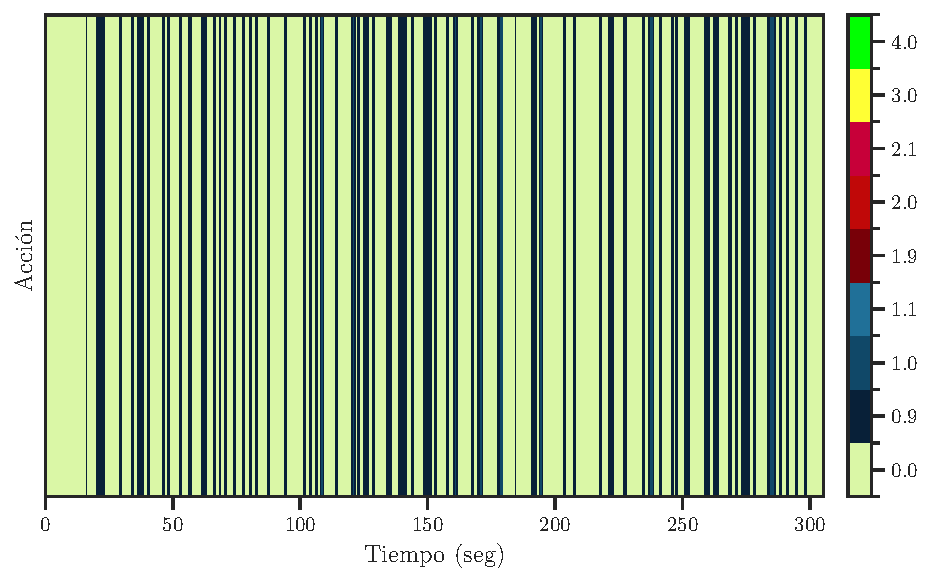
\includegraphics[width=\imsize]{accion_aleatorio.pdf}
	\caption[ Matriz de Acciones de un Conectoma Aleatorio.]{ Matriz de Acciones de un Conectoma Aleatorio. La Figura  muestra la matriz de acciones resultante de experimentos con un conectoma aleatorio. Los patrones de comportamiento del robot en este contexto carecen de coherencia y complejidad, predominando movimientos repetitivos sin respuestas coordinadas.  }\label{fig:comportamiento_aleatorio}
\end{figure}


\begin{figure}[h!]
	\centering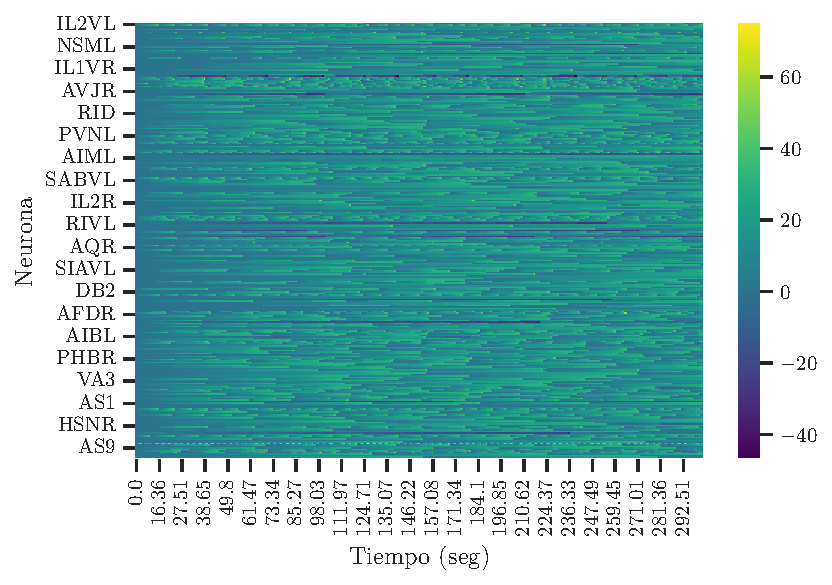
\includegraphics[width=\imsize]{matriz_valores_aleatorio.pdf}
	\caption[ Dinámica Neuronal en un Conectoma Aleatorio.]{ Dinámica Neuronal en un Conectoma Aleatorio.  En la Figura, se presenta la dinámica neuronal correspondiente a un conectoma aleatorio. Observamos la falta de grupos de neuronas sincronizadas, en contraste con lo que se esperaría encontrar en un organismo complejo como el C. elegans. }\label{fig:comportamiento_aleatorioneurona}
\end{figure}



En contraste, cuando el robot opera con la dinámica neuronal que contiene el conectoma del C. elegans, exhibe un comportamiento rico y complejo. Por ejemplo, cuando se enfrenta a un obstáculo, retrocede, emulando así el comportamiento del gusano real (véase la \Cref{fig:acciones} de la matriz de acciones en un experimento de 20 minutos). Además, en la dinámica neuronal se observan grupos de neuronas sincronizadas, tal como se muestra en la Figura 4, los cuales son comparables a los encontrados en experimentos con el C. elegans real (véase la \Cref{fig:kato} de un experimento con C. elegans realizado por Kato et al. \cite{kato_global_2015}).


\subsubsection{Discusión}

Los resultados previos son de relevancia, ya que si el comportamiento del robot con un conectoma aleatorio fuera idéntico al observado con el conectoma real, se podría argumentar que el comportamiento resulta de casualidades u otros factores, lo cual invalidaría cualquier análisis posterior. Afortunadamente, el comportamiento complejo, caracterizado por la exploración del entorno y respuestas a estímulos, solo emerge en una red compleja con características topológicas complejas, como el conectoma del C. elegans. El hecho de que la aleatoriedad no produzca un comportamiento coherente en el robot respalda la hipótesis de que el conectoma del C. elegans codifica de alguna manera parte de su comportamiento motor, posiblemente a través de la evolución, restricciones energéticas, genética o una combinación de estos factores. 

Recientemente, Azulay et al. \cite{azulay_c_2016} respaldaron esta hipótesis al revelar, mediante simulaciones de propagación de señales, que la red del C. elegans desempeña roles funcionales específicos. En áreas definidas de la red neuronal, se encuentran conjuntos homogéneos especializados que funcionan como bloques de construcción para llevar a cabo diversas tareas de procesamiento. Por ejemplo, los conjuntos homogéneos que se regulan mutuamente respaldan la integración, la memoria a corto plazo y la amplificación de señales en las capas sensoriales e interneuronales, mientras que los conjuntos homogéneos que se regulan mutuamente sincronizan múltiples entradas de neuronas comunes ascendentes para respaldar la actividad coordinada del sistema motor. Estas características no están presentes en una red aleatoria.  








\section{Comportamiento de la dinámica neuronal Global}



Se realizaron experimentos de $\sim$ 20 minutos de duración en un entorno experimental controlado. El gusano se coloco en una caja cuadrada de \qty{1}{\m^2}. En cada paso de tiempo, se realizaron registros en archivos separados de las variables más importantes, como se describe a continuación:

\begin{itemize}
	\item \textbf{Registro de actividad neuronal: } Este registro almacena los valores acumulados en ese tiempo dado de cada neurona. A partir de este registro, se generó un fichero final que muestra cómo varía la actividad neuronal en función del tiempo de cada una de las neuronas que compone el conectoma. Los datos se almacenaron en formato CSV, con cada fila representando un registro de actividad neuronal. Cada registro contiene los siguientes campos:
	
	\begin{itemize}
\item  	\textbf{Neurona:} El identificador de la neurona.
\item  \textbf{Tiempo: } El tiempo de la medición.
\item \textbf{Valor: }El valor de la actividad neuronal.
	\end{itemize}
		
	\item \textbf{Registro de acciones motoras:} Este registro almacena las acciones realizadas por el motor del robot en ese tiempo dado. Los valores numéricos de estas acciones se asignaron de acuerdo con el  \Cref{table:accioens_robot}. Los datos se almacenaron en formato CSV, con cada fila representando un registro de acciones motoras. Cada registro contiene los siguientes campos:
	
\begin{itemize}
\item \textbf{	Acción:} El tipo de acción.
\item \textbf{Tiempo:} El tiempo de la medición.
\end{itemize}
	\item \textbf{Registro de tiempo de simulación:} Este registro almacena el tiempo de simulación (iteraciones). Los datos se almacenaron en formato CSV, con cada fila representando un registro de tiempo de simulación. .
	\item \textbf{Registro de tiempo real:} Este registro almacena el tiempo real.
	\item \textbf{Registro de valor del sensor:} Este registro almacena el valor del sensor en cada instante de tiempo.
\end{itemize}

\begin{table}[h!]
	\centering
	\caption[Acciones registradas en el robot. ]{ Acciones registradas en el robot.	}
	\begin{tblr}{colspec={ll},
			row{odd} = {bg=gray8},
			row{even} = {bg=gray9},
			row{1} = {bg=red3, fg=white, font=\sffamily},
		}
		
		Acción	& Valor\\
		Detenido &	0.0 \\
		Marcha atrás izquierda &	0.9 \\
		Marcha atrás &	1.0 \\
		Marcha atrás derecha& 	1.1 \\
		Marcha adelante izquierda &	1.9 \\
		Marcha adelante	& 2.0\\
		Marcha adelante derecha	& 2.1\\
		Rotar derecha	& 3.0\\
		Rotar izquierda	& 4.0\\
	\end{tblr}
	\label{table:accioens_robot}
\end{table}



En general, el robot  que utiliza el conectoma artificial se comportó de forma muy similar a los comportamientos observados en el C. elegans biológico. En los términos más simples, la estimulación de las neuronas sensoriales de los alimentos provocó que el robot se moviera hacia adelante. Este comportamiento esta documentado en animales reales. La búsqueda restringida a un área (ARS) es una estrategia de alimentación universal bien descrita en la que los animales giran con más frecuencia después de un encuentro con la comida para restringir su búsqueda localmente. A medida que aumenta el período de tiempo desde el último encuentro con la comida, los animales giran con menos frecuencia y comienzan a moverse hacia nuevas áreas. Esto tiene sentido ecológico: los animales aprenden que la comida no está agrupada cerca y por lo tanto se mueven para buscar nuevas fuentes de alimentos. La ARS también se observa en C. elegans \cite{flavell_dynamic_2022}.  Por lo tanto, si un gusano que se está alimentando se transfiere a un entorno sin comida, inicialmente realiza movimientos de avance de corta duración y giros de alto ángulo. Si hay comida cerca, este comportamiento aumenta la probabilidad de que el gusano vuelva a encontrarla. Si no hay comida cerca, durante un cierto período  de tiempo, el comportamiento del gusano cambia de tal manera que la duración del movimiento hacia adelante aumenta y la probabilidad de reversos o giros de alto ángulo disminuye. Al analizar el comportamiento del robot sin ningún obstáculo (las neuronas del hambre son estimuladas), la proporción de  veces qe el robot realiza acciones de avances hacia adelante compara con los de avance hacia atrás es mayor.  Como se menciono anteriormente este comportamiento en el robot  esta en concordancia con lo encontrado en animales reales.   


La estimulación del sensor láser  del robot, que a su vez estimulaba las neuronas táctiles de la nariz, hacía que el robot detuviera su movimiento hacia adelante, retrocediera y luego siguiera adelante, normalmente en una trayectoria ligeramente sesgada.  Al igual que en el caso anterior el comportamiento es similar al de C. elgans reales. Los  C. elegans responden al tacto suave en la nariz iniciando la locomoción hacia atrás \cite{chalfie_assaying_2018,chalfie_neural_1985}. Esta respuesta se denomina \textquote{Respuesta al tacto en la nariz} o ensayo Not.  

No hay ningún programa que dirija al robot a comportarse de una manera específica. Solo el conectoma simulado dicta cuándo el robot moverá un motor hacia adelante, se detendrá o retrocederá. Esto podría responde, a un nivel muy básico, que el conectoma (es decir, cómo está cableado un sistema nervioso)  junto con una dinámica neural sencilla  podría dar lugar a los fenotipos que observamos en los animales. El  video suplementario 1 (\url{https://www.frontiersin.org/articles/10.3389/fnbot.2022.1041410/full#supplementary-material}) muestra al robot utilizando el conectoma y el sistema nervioso simulado de C. elegans.  La parte central del video muestra al robot cuando se acerca a una pared, activa las neuronas sensoriales táctiles de la nariz, se detiene y cambia de dirección, de nuevo totalmente bajo el control del sistema nervioso del C. elegans simulado. La repetición de estos experimentos arrojó resultados similares una y otra vez. El conectoma de C. elegans es altamente recursivo. Cuando el conectoma alcanza un nivel suficiente de estimulación, se autoestimula continuamente: una neurona (presináptica) estimula a otro conjunto de neuronas (postsinápticas), y a su vez, muchas de esas neuronas postsinápticas estimulan a la neurona presináptica original, creando bucles de estimulación. La naturaleza recursiva del conectoma ha demostrado ser un factor clave en la investigación del connectoma y los comportamientos resultantes de C. elegans. Se ha determinado que, si se deja solo, el conectoma simulado de C. Elegans, o su sistema nervioso, funcionará continuamente para siempre sin necesidad de más estimulación. Esto no es diferente de los cerebros biológicos de los animales, donde la actividad cerebral se observa constantemente incluso en estados de inconsciencia profunda. Como trabajo futuro se podría realizar una análisis utilizando medidas y herramientas de la teoría de grafos y  redes complejas  para determinar cómo estos bucles recursivos juegan en la topología y las acciones resultantes cuando el conectoma está totalmente comprometido.


\section{Neuronas Estimuladas y Comportamiento del Robot}\label{sec:estimuladas}


Este apartado se dedica a analizar la relación entre las neuronas estimuladas, es decir, los circuitos neuronales, y las respuestas ejecutadas por el robot. Es importante mencionar que nuestro modelo actual se encuentra limitado en su repertorio de acciones debido a su configuración de dos ruedas y un único sensor.  Para establecer una conexión efectiva entre la actividad neuronal y el comportamiento del robot, diseñamos una serie de experimentos que abarcan tres intervalos de tiempo:

\begin{itemize}
\item \textbf{Exploración Sin Obstáculos: } En el primer intervalo, el robot se movió libremente por un espacio sin obstáculos durante un período de 5 minutos, estimulando únicamente las neuronas relacionadas con el hambre.
\item \textbf{Reacción a Obstáculos: }  En el segundo intervalo de 5 minutos, el robot se posicionó frente a un obstáculo, desencadenando la estimulación de las neuronas responsables de la percepción táctil en la nariz.
\item \textbf{Entorno Complejo:} Finalmente, el robot volvió a moverse en un entorno con obstáculos, simbolizando un escenario más complejo
\end{itemize}

El propósito fundamental de estos experimentos reside en examinar cómo el comportamiento del robot se adapta a la estimulación de neuronas específicas. En el primer intervalo, la estimulación se concentró en las neuronas del hambre, que incluyeron ADFL(R), ASGL(R), ASIL(R) y ASJL(R). Estas neuronas están vinculadas a circuitos neuronales que guían la exploración y búsqueda de alimentos. En el organismo modelo, el C. elegans, la activación de estas neuronas induce movimientos hacia adelante y exploración del entorno, con episodios ocasionales de marcha atrás. La \Cref{fig:intervalos_hambre} presenta la dinámica neuronal de estas neuronas del hambre en los tres intervalos previamente mencionados, con el intervalo de obstáculos resaltado en azul. Se observa que algunas neuronas, como ADFL(R), experimentaron un cambio de oscilación de frecuencia baja a alta cuando se encontraron con un obstáculo, mientras que otras, como ASIL(R) y ASJL(R), manifestaron un efecto inverso, con una disminución de la frecuencia. La actividad de ASGL(R) se mantuvo constante en todos los intervalos. Este resultado resalta la adaptabilidad de la dinámica neuronal en respuesta a cambios en el entorno, sugiriendo que el robot ajusta su comportamiento en función de estas variaciones, con la dinámica neuronal modulando dicho comportamiento.

\begin{figure}[h!]
	\centering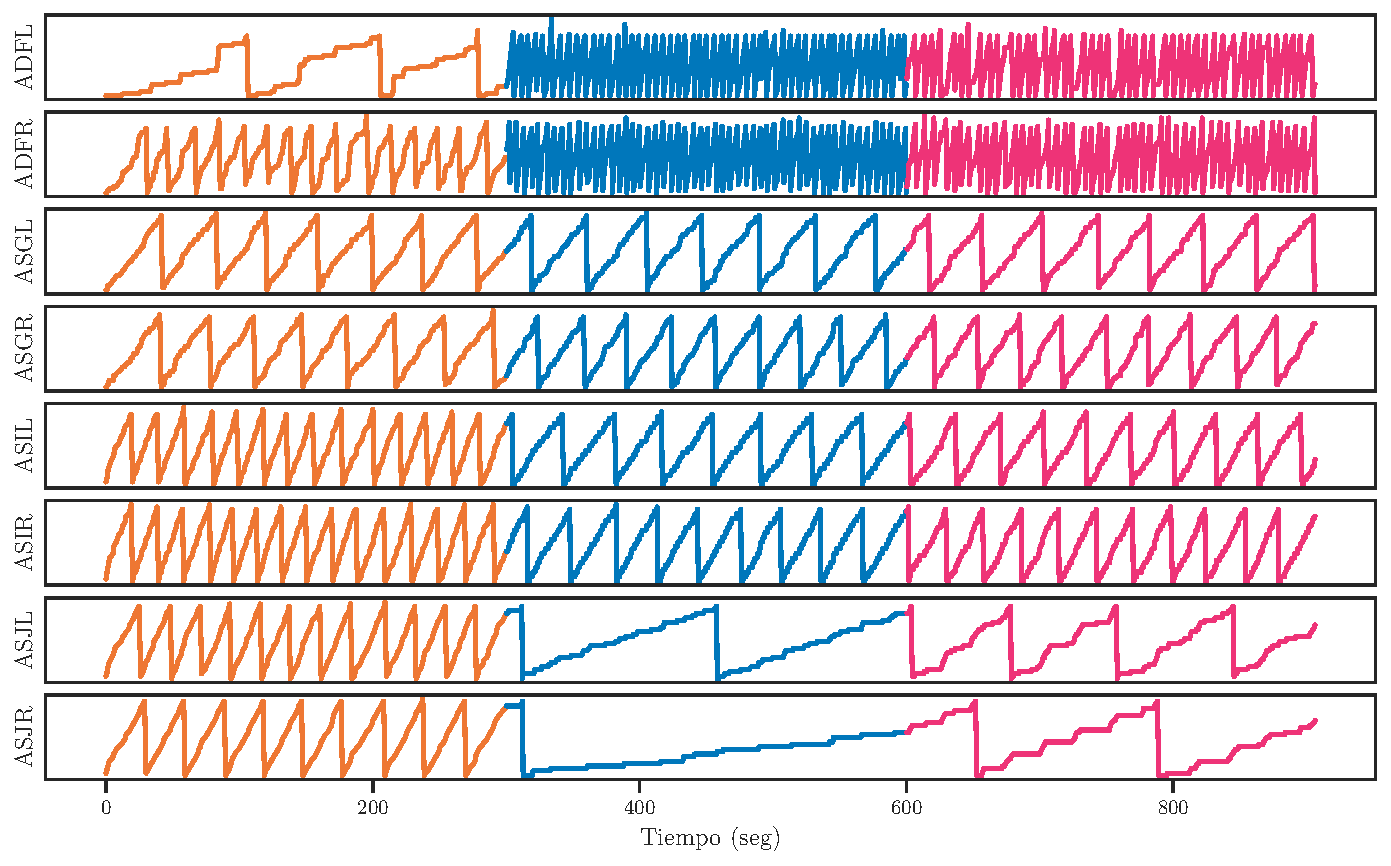
\includegraphics[width=\imsize]{intervalos_hambre.pdf}
	\caption[   Dinámica Neuronal de las Neuronas del Hambre en Tres Intervalos de Tiempo. ]{  Dinámica Neuronal de las Neuronas del Hambre en Tres Intervalos de Tiempo. La figura muestra cómo la frecuencia de oscilación de neuronas como ADFL(R), ASIL(R), y ASJL(R) varía en respuesta a diferentes entornos. El intervalo en el que el robot se encuentra frente a un obstáculo se destaca en azul, revelando cambios notables en la dinámica neuronal debido a la alteración del ambiente. }\label{fig:intervalos_hambre}
\end{figure}

En el segundo intervalo, se estimularon las neuronas de percepción táctil en la nariz, que incluyeron FLPR(L), ASHL(R), IL1VL(R), OLQDL(R) y OLQVR(L). Estas neuronas desencadenan movimientos de retroceso en el C. elegans en caso de colisión con un objeto. Tres clases de neuronas mecanosensoriales (ASH, FLP y OLQ) operan en paralelo para mediar esta respuesta, contribuyendo en fracciones distintas a la respuesta global: ASH (45\%), FLP (29\%) y OLQ (5\%). Las respuestas restantes ($\sim$10\%) son mediadas por las neuronas ALM y AVM, que detectan el tacto en la parte anterior del cuerpo. En el experimento con el robot, cuando se enfrenta a una pared y se activan estas neuronas, el robot ejecuta movimientos de retroceso para evitar el obstáculo. La \Cref{fig:intervalos_nariz} ilustra la actividad de estas neuronas, con el intervalo en el que el robot se encuentra frente a un obstáculo coloreado de azul. Al igual que en el caso de las neuronas del hambre, el impacto de la pared provoca un aumento en la frecuencia de algunas neuronas, como FLPR(L), ASHL, IL1VL(R) y OLQDL(R), mientras que ASHR mantiene su actividad inalterada. El último intervalo de tiempo refleja un comportamiento similar al descrito en el apartado anterior, donde el robot se adapta al entorno. Este intervalo se identifica visualmente mediante el color rosa.

\begin{figure}[h!]
	\centering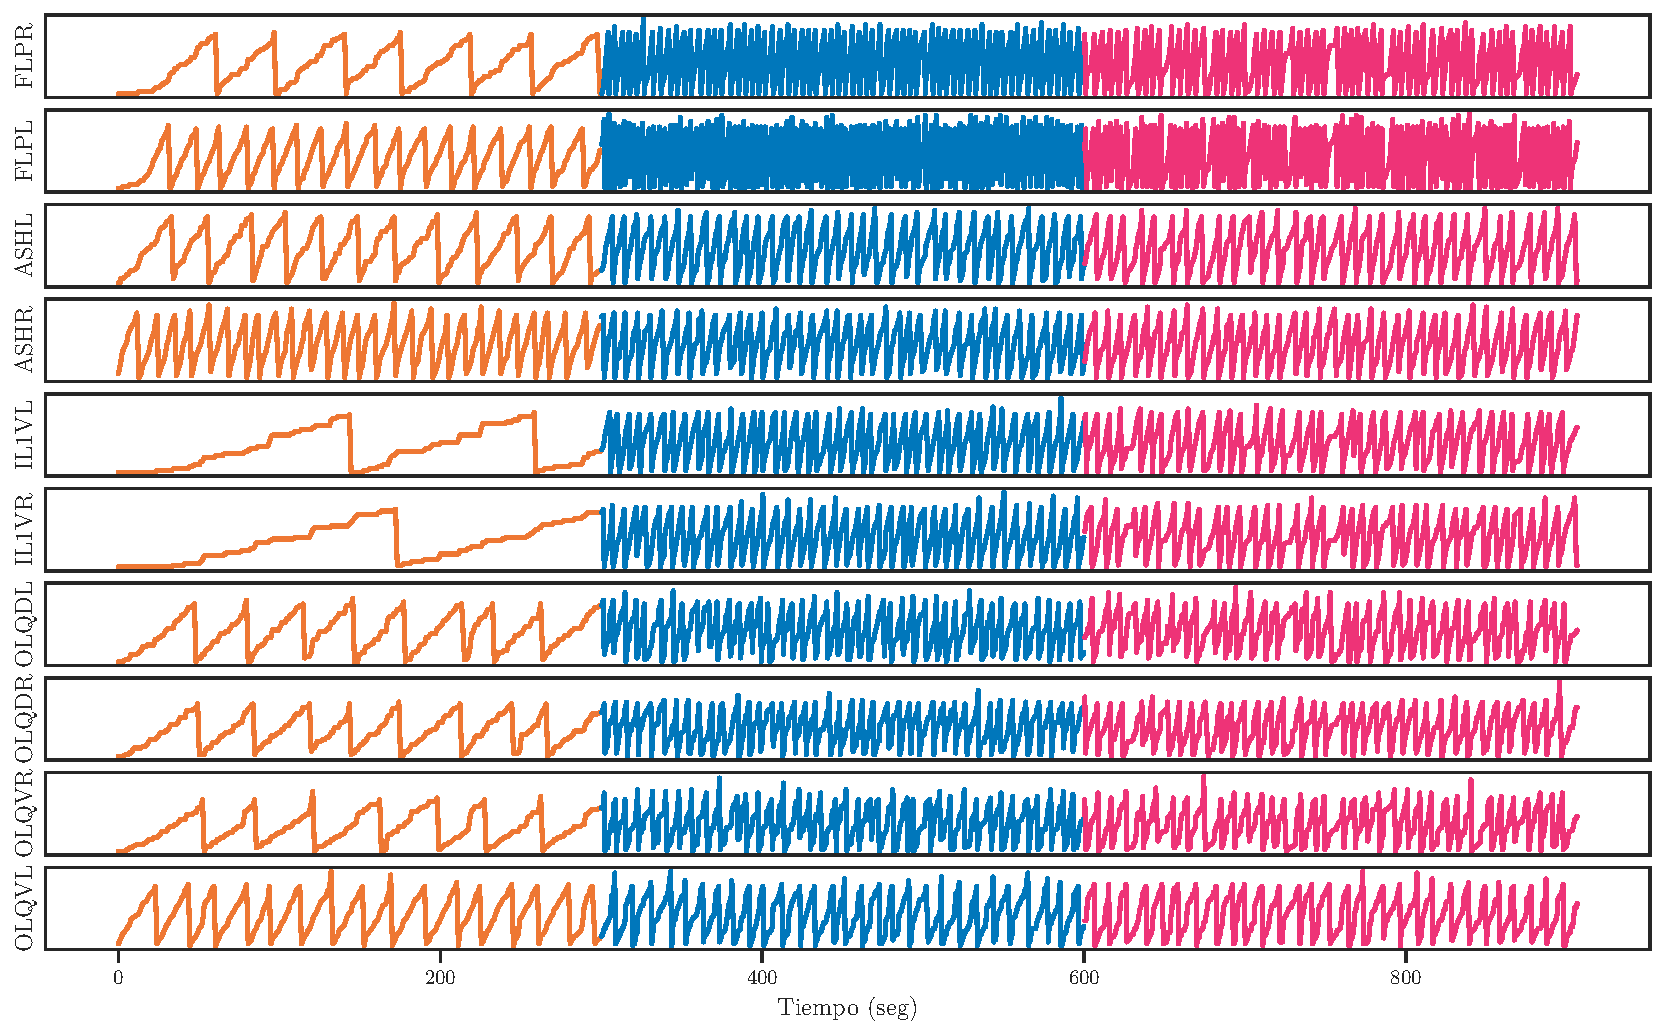
\includegraphics[width=\imsize]{intervalos_nariz.pdf}
	\caption[    Actividad Neuronal en el Segundo Intervalo con Estimulación de Neuronas de Tacto en la Nariz.  ]{   Actividad Neuronal en el Segundo Intervalo con Estimulación de Neuronas de Tacto en la Nariz.  En el intervalo en el que el robot se coloca frente a un obstáculo (resaltado en azul), se observa cómo las neuronas, como FLPR(L), ASHL, IL1VL(R), y OLQDL(R), experimentan cambios en su frecuencia de actividad en respuesta a la percepción táctil. La neurona ASHR, en cambio, mantiene su actividad constante.}\label{fig:intervalos_nariz}
\end{figure}

Para validar que el comportamiento emergente del robot se asemeja a lo observado en la biología del C. elegans, registramos las frecuencias de las acciones de avance, retroceso y rotación en la duración de los dos primeros intervalos. En el primer intervalo, donde solo se estimularon las neuronas del hambre (intervalo 1), predominaron las acciones de avanzar, en línea con la tendencia de los gusanos reales a explorar en busca de alimentos cuando se encuentran en un entorno rico en comida. En el caso de nuestro neuro-robot, el comportamiento fue análogo, con la mayor parte del tiempo destinado a avanzar y girar, explorando el espacio. Este patrón se refleja en las barras de la \Cref{fig:intervalo_comportamiento}a, donde las acciones relacionadas con el avance son más frecuentes que las demás. Por otro lado, en el segundo intervalo, se sabe que los gusanos reales tienden a huir de cualquier contacto, debido a su exposición a depredadores, como lo demuestran experimentos con pelos microscópicos. Por lo tanto, se esperaba que las acciones predominantes fueran las de retroceso, lo que se confirma en la \Cref{fig:intervalo_comportamiento}b, donde las acciones relacionadas con el retroceso son las más frecuentes.  Estos resultados indican que la dinámica cerebral modula el comportamiento del robot en función de las neuronas estimuladas, lo que refleja la adaptación del robot al entorno.

\begin{figure}[h!]
	\centering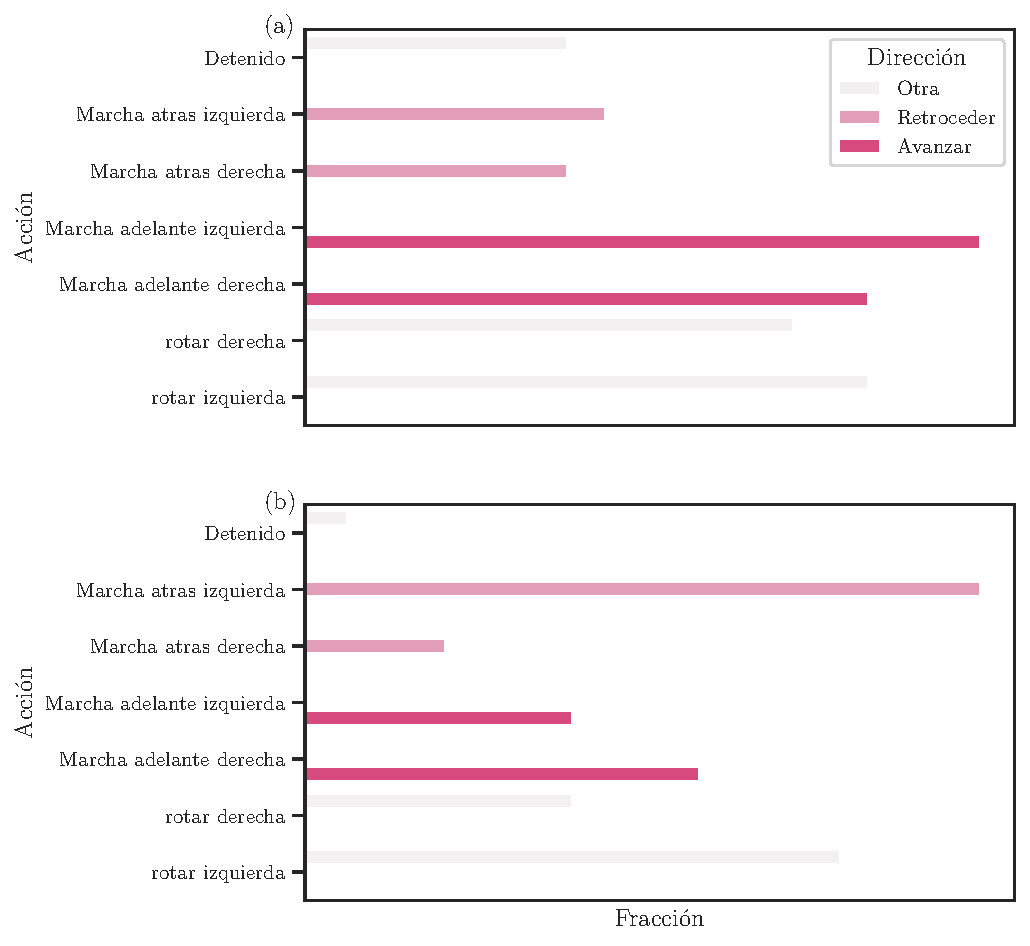
\includegraphics[width=\imsize]{fraccion_acciones.pdf}
	\caption[  Frecuencia de Acciones del Robot en el Primer y Segundo Intervalo.]{ Frecuencia de Acciones del Robot en el Primer y Segundo Intervalo.  (a) En el intervalo 1, con solo la estimulación de las neuronas del hambre, predominan las acciones de avanzar, reflejando la exploración en busca de alimentos, similar a lo observado en gusanos reales en entornos ricos en comida. (b) En el intervalo 2, cuando se estimulan las neuronas de percepción táctil en la nariz, las acciones de retroceso son prominentes, concordando con la tendencia de los gusanos reales a retroceder ante cualquier contacto debido a la presencia de posibles depredadores.}\label{fig:intervalo_comportamiento}
\end{figure}




\subsection{Discusión}

A pesar de contar únicamente con dos circuitos implementados en nuestro robot, hemos logrado obtener una amplia variedad de comportamientos complejos. Cabe destacar que en ningún momento se han programado órdenes específicas; en su lugar, se han activado los circuitos de mayor relevancia que previamente se habían identificado mediante ablación láser y otros experimentos. Para ampliar aún más el repertorio de comportamientos complejos, podríamos considerar la incorporación de más sensores y, basándonos en los hallazgos de la biología, activar los circuitos correspondientes. Por ejemplo, podríamos implementar un circuito relacionado con la detección de toques bruscos en el cuerpo a través de sensores táctiles. La implementación de hardware podría consistir en dos sensores táctiles, uno en la parte anterior y otro en la posterior del robot, cada uno con una entrada simple que puede estar "encendida" o "apagada". Cuando se presiona un sensor táctil, envía una señal de "encendido" que es leída por el programa de entrada. Si el sensor no se encuentra presionado (apagado), este envía una señal de "apagado". La activación de este sensor desencadenaría los circuitos relacionados con la percepción de toques bruscos, tanto en la parte anterior como en la posterior del robot. En el caso del C. elegans, la detección de toques bruscos en el cuerpo provoca una respuesta de retroceso marcada en el gusano. Sería interesante explorar si este modelo de conectoma puede reproducir el comportamiento cualitativo de orientación, tal como se investigó en el estudio de Morse et al. (1998), utilizando un sensor de luz.

El C. elegans localiza alimentos a través de la quimiotaxis, la capacidad de orientarse en respuesta a gradientes de concentración química. Sería valioso investigar si podemos observar un comportamiento de orientación similar a la quimiotaxis en nuestro modelo. Con un conjunto adecuado de sensores y una implementación precisa, podríamos estudiar circuitos neuronales asociados con comportamientos complejos en el robot de manera relativamente sencilla. Esto representa una ventaja significativa en comparación con los gusanos reales, ya que nos brinda acceso completo a la dinámica del sistema.

A pesar de las limitaciones actuales, este enfoque promete una mayor comprensión de los circuitos neuronales y del comportamiento emergente en los robots. Para lograr una mayor diversidad de comportamientos complejos, podríamos considerar la incorporación de más sensores y la activación de circuitos adicionales, lo que nos permitiría explorar una variedad de comportamientos complejos.





\section{La actividad neuronal global evoluciona en un colector de dimensión baja similar a un atractor}

La comprensión de cómo el sistema nervioso codifica, organiza y secuencializa los comportamientos es un pilar fundamental en la neurociencia de sistemas, ya sea al estudiar organismos tan simples como los gusanos o tan complejos como los seres humanos. En este contexto, nuestro estudio se enfoca en la evaluación de la relación entre la dinámica neuronal en el gusano C. elegans y su comportamiento, empleando técnicas experimentales afines a las utilizadas por Kato et al., cuyos resultados se presentan de manera resumida en la \Cref{sec:dinamicakato} y se ilustran en la \Cref{fig:kato}.

Con el propósito de abordar esta cuestión, llevamos a cabo un experimento que se extendió aproximadamente durante 20 minutos. Durante este período, el neurorobot emuló la actividad neuronal de C. elegans en el montaje experimental previamente descrito. Los datos resultantes comprenden 300 series temporales de datos dimensionales que detallan la actividad neuronal, con una dimensión asociada a cada neurona. La complejidad inherente de estos datos plantea un desafío inicial para su comprensión, lo que motiva la necesidad de un análisis más sofisticado.

En la \Cref{fig:matrizrobot}, se presenta la matriz de actividad que captura la dinámica neuronal del robot. Para identificar grupos de neuronas sincronizadas, implementamos un algoritmo de agrupación jerárquica utilizando la función \textbf{clustermap} de la biblioteca Seaborn. Esta aproximación nos permitió de manera efectiva visualizar la estructura subyacente en los datos y discernir los patrones de sincronización neuronal que son esenciales para comprender la relación entre la actividad neuronal y el comportamiento del neurorobot.


 \begin{figure}[h!]
	\centering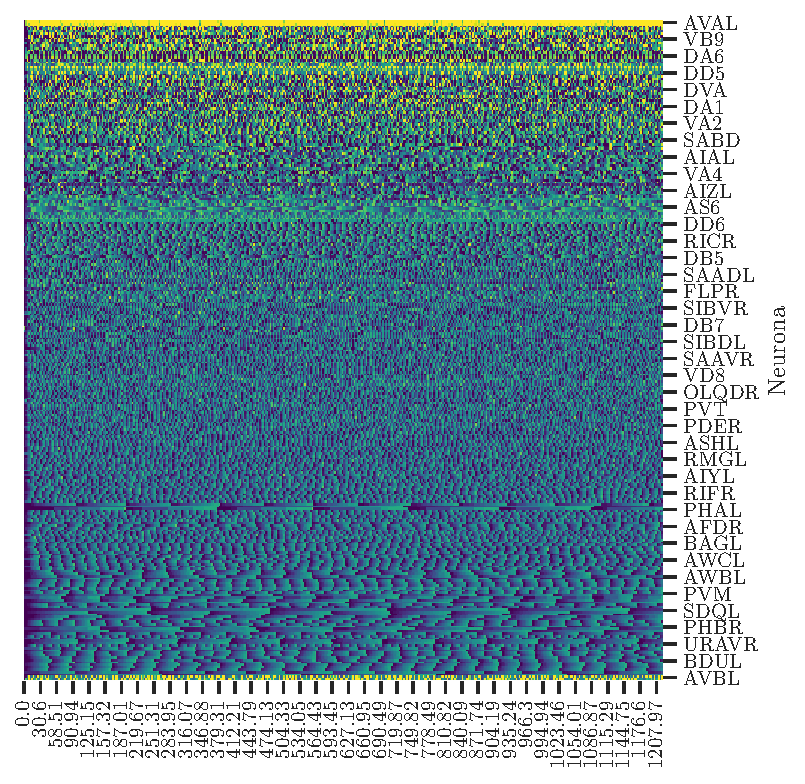
\includegraphics[width=\imsize]{clusteres_dinamica.pdf}
	\caption[ Matriz de Actividad que Representa la Dinámica Neuronal del Neurorobot.]{ Matriz de Actividad que Representa la Dinámica Neuronal del Neurorobot. Se muestra la matriz de actividad que refleja la dinámica neuronal del neurorobot durante el experimento. Cada entrada de la matriz corresponde a la actividad de una neurona en un instante de tiempo específico. Utilizando un algoritmo de agrupación jerárquica, se identificaron patrones de sincronización entre las neuronas, lo que proporciona una visión crucial de la coordinación neuronal en el sistema. Este análisis de la dinámica neuronal es fundamental para comprender la relación entre la actividad neuronal y el comportamiento emergente del neurorobot.}\label{fig:matrizrobot}
\end{figure}



 \begin{figure}[h!]
	\centering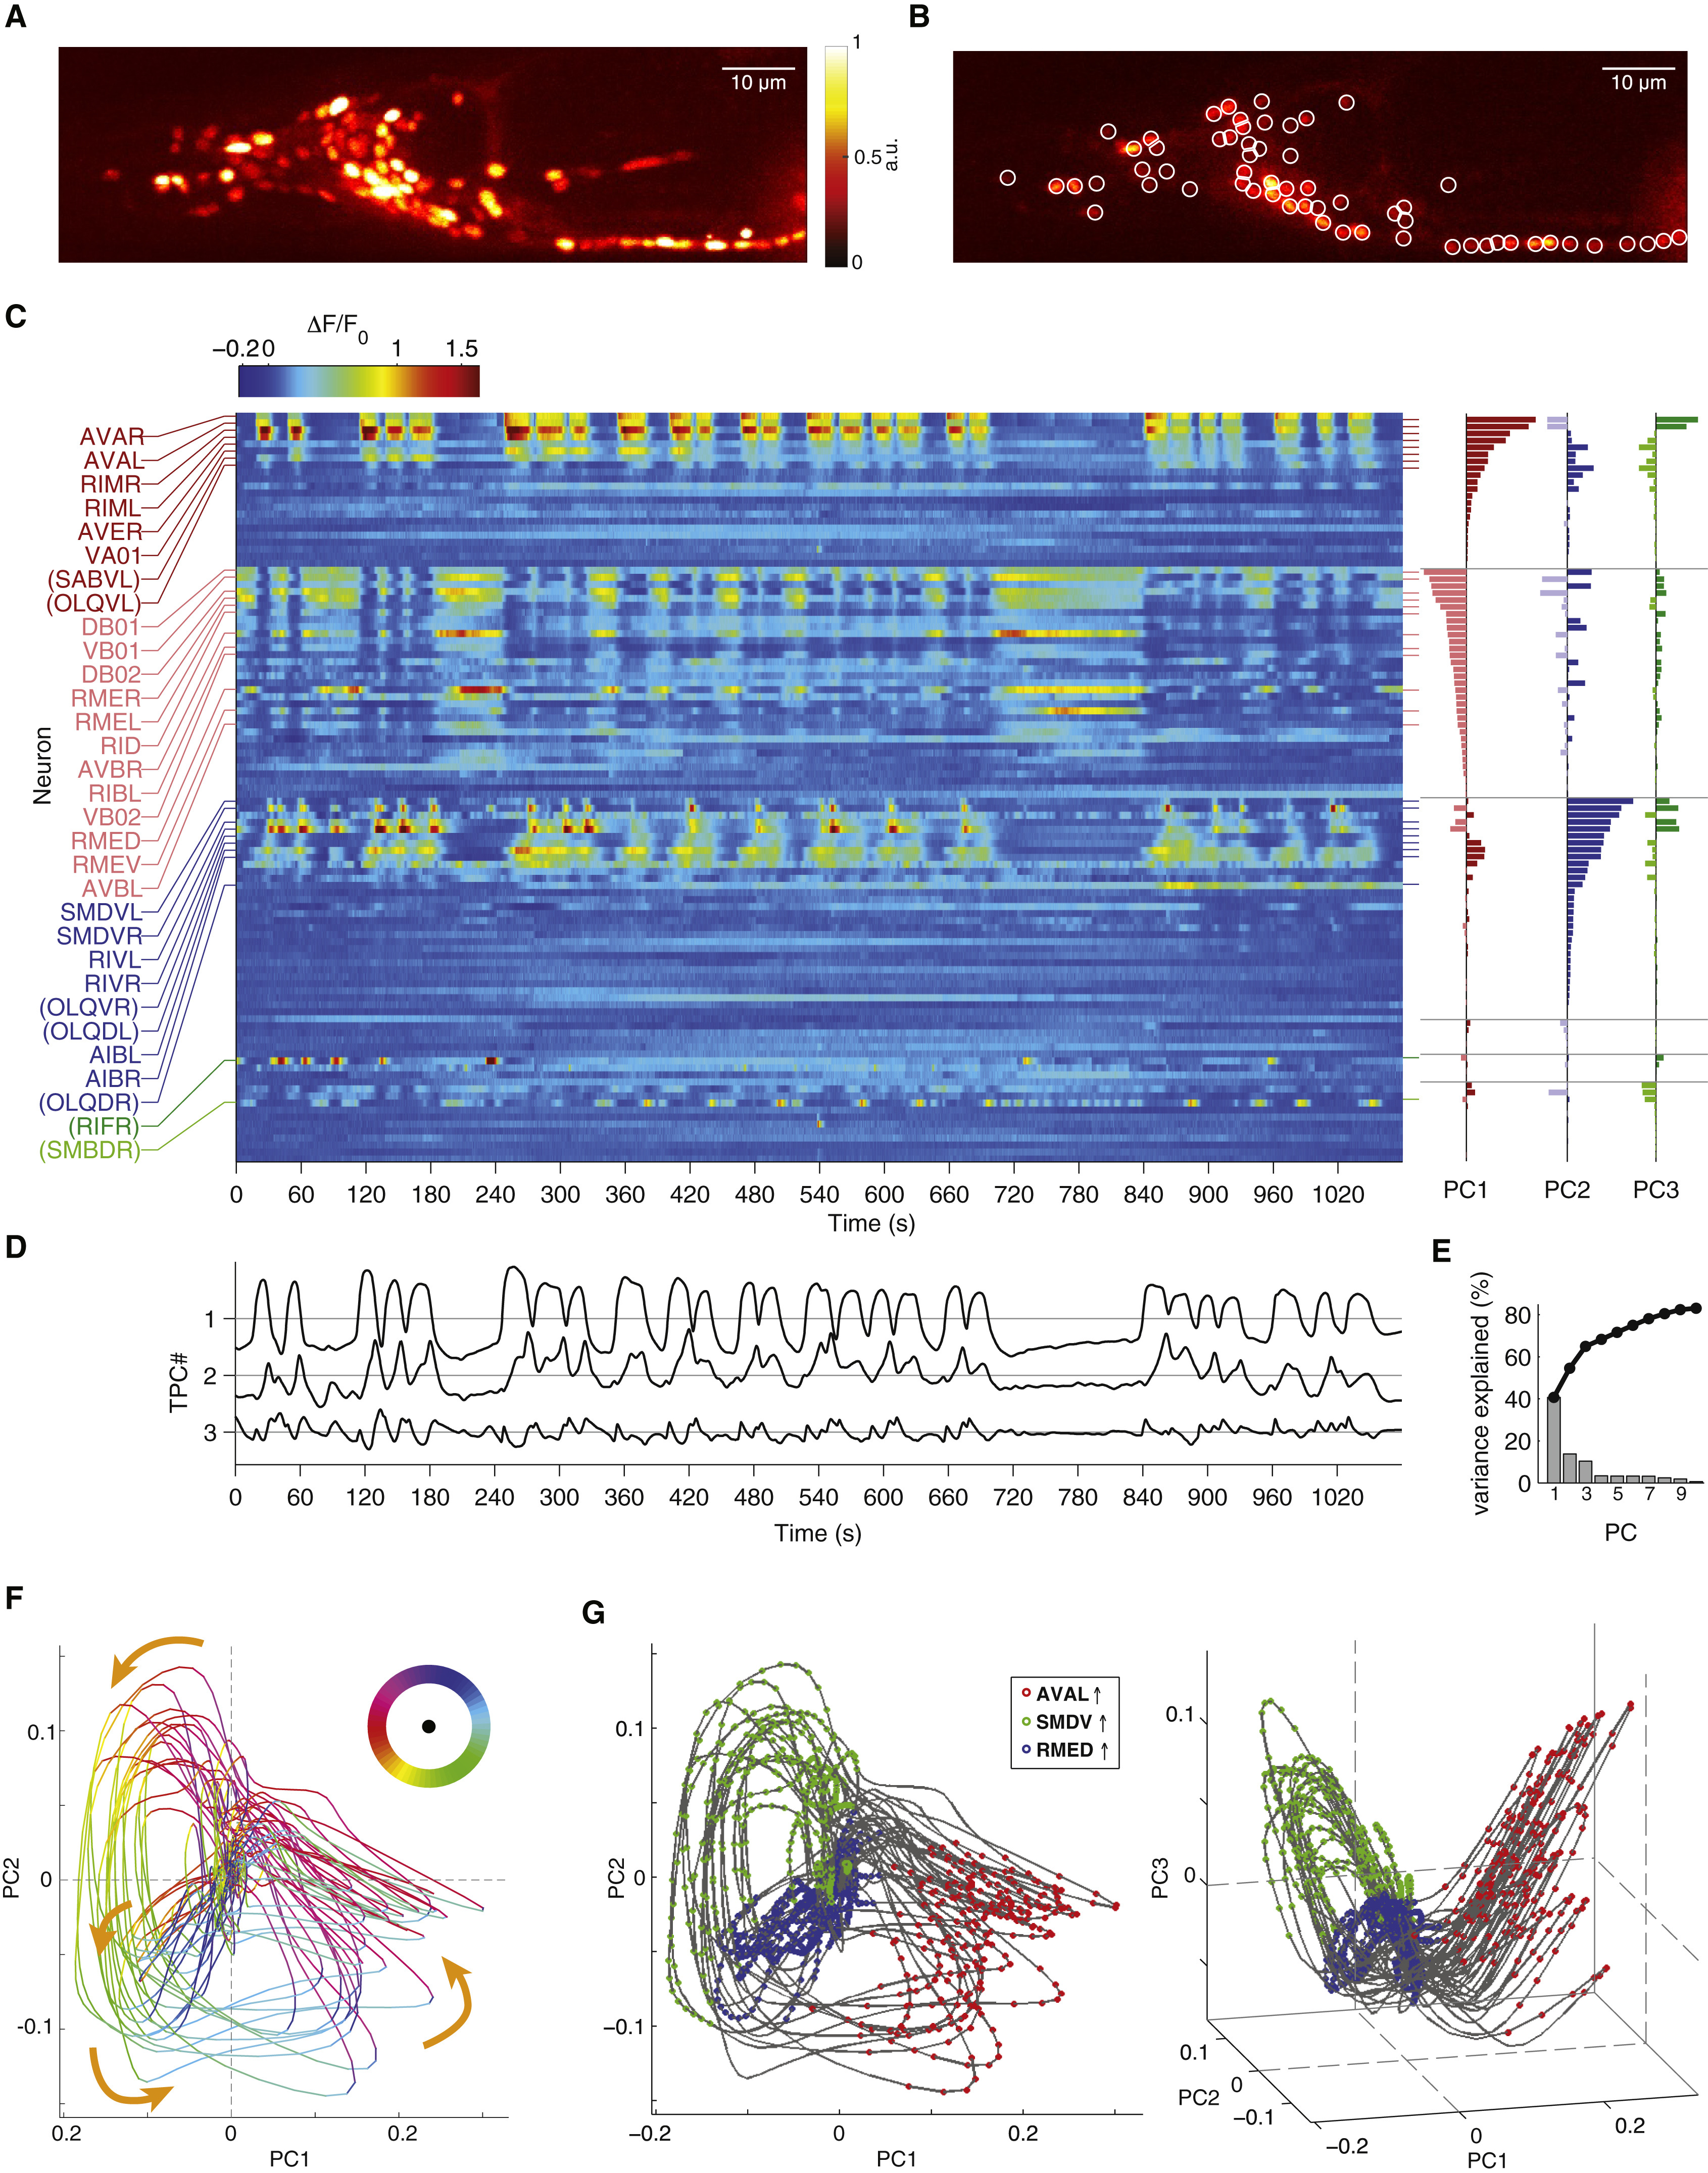
\includegraphics[width=\imsize]{kato.jpg}
	\caption[ La actividad cerebral se organiza en una trayectoria de espacio de estado neural cíclico de baja dimensión en gusanos reales.]{ La actividad cerebral se organiza en una trayectoria de espacio de estado neural cíclico de baja dimensión en gusanos reales.  (A) Proyección de máxima intensidad de una muestra representativa grabada en condiciones constantes.
		(B) Plano z único superpuesto con regiones neuronales segmentadas.
		(C) Mapa de calor de las series de tiempo de fluorescencia ($\Delta F/F$) de 109 neuronas cefálicas segmentadas, una neurona por fila.  Las neuronas están coloreadas y agrupadas por sus pesos y signos de componentes principales (PC1-3), que se muestran en los gráficos de barras de la derecha. (D) Integrales de los tres primeros PC temporales. (E) Varianza explicada por los primeros diez PC, la línea negra indica la varianza acumulada explicada. 		(F) Diagrama de fase de los dos primeros PC temporales coloreados por la dirección de la evolución temporal indicada por la leyenda de colores. (G) Diagramas de fase de los dos primeros (izquierda) y los tres primeros (derecha) PC temporales. }\label{fig:kato}
\end{figure}




 Dado que los datos son ruidosos, aplicamos una derivada temporal a nuestra matriz de actividad neuronal, utilizando una derivada regularizada (\Cref{eq:ap:2}) con un parámetro de regularización $\alpha$ de 2 (\Cref{fig:derivada_regularizada}). Luego, estandarizamos los datos, lo que implica transformarlos para que sigan una distribución normal estándar (gaussiana) con una media de cero y una varianza unitaria. Esta estandarización es un requisito común para muchos algoritmos de aprendizaje automático, como el Análisis de Componentes Principales (PCA).  Luego de estandarizar los datos, realizamos un análisis de componentes principales (PCA) de las derivadas temporales de las trazas normalizadas, lo que nos permitió proyectar los datos originales de 301 dimensiones en tres dimensiones. Estos nuevos componentes representan las tres dimensiones principales de la variación, como se ilustra en la \Cref{fig:pcs}. Además, para cada componente principal (PC), generamos una serie temporal correspondiente (PC temporal) al calcular la media ponderada de la serie temporal multineural completa. Los PC temporales capturan señales compartidas por neuronas que se agrupan en función de sus correlaciones. De manera sorprendente, descubrimos que los tres primeros PC explicaban el 30 \% de la varianza total en nuestros datos, como se muestra en la \Cref{fig:varianza}.
 
 
  \begin{figure}[h!]
 	\centering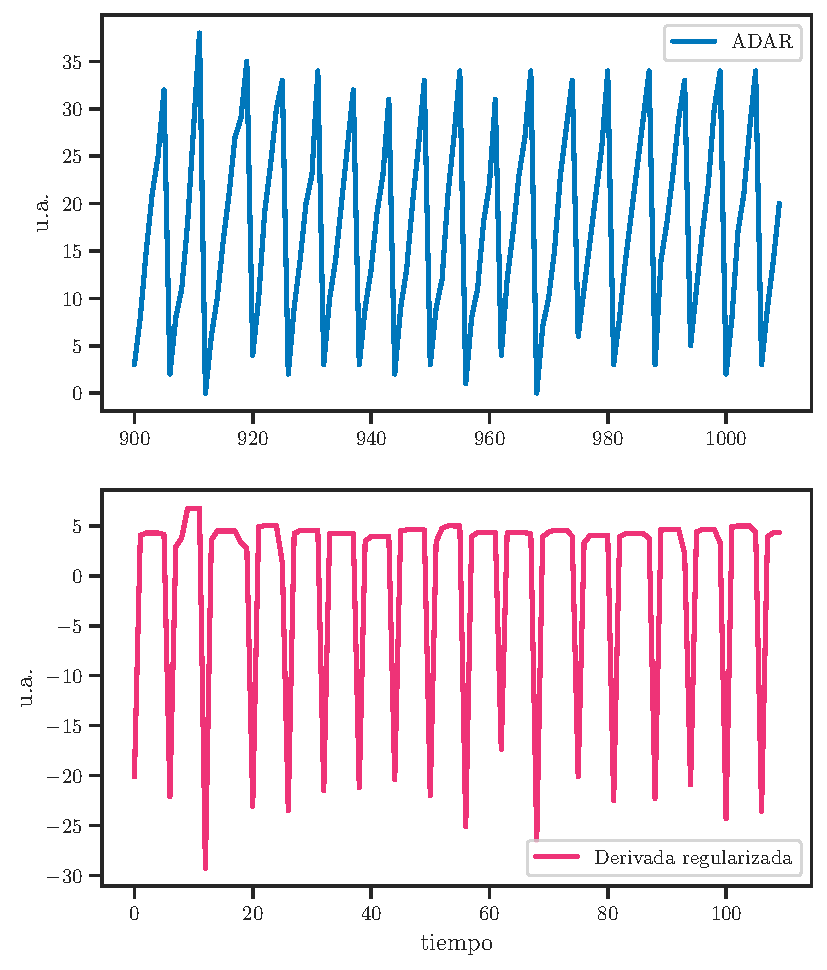
\includegraphics[width=\imsize]{derivada_robot.pdf}
 	\caption[Ejemplo de aplicar la derivada regularizada a una neurona del experimento.]{Ejemplo de aplicar la derivada regularizada a una neurona del experimento.}\label{fig:derivada_regularizada}
 \end{figure}
 
 
 \begin{figure}[h!]
 	\centering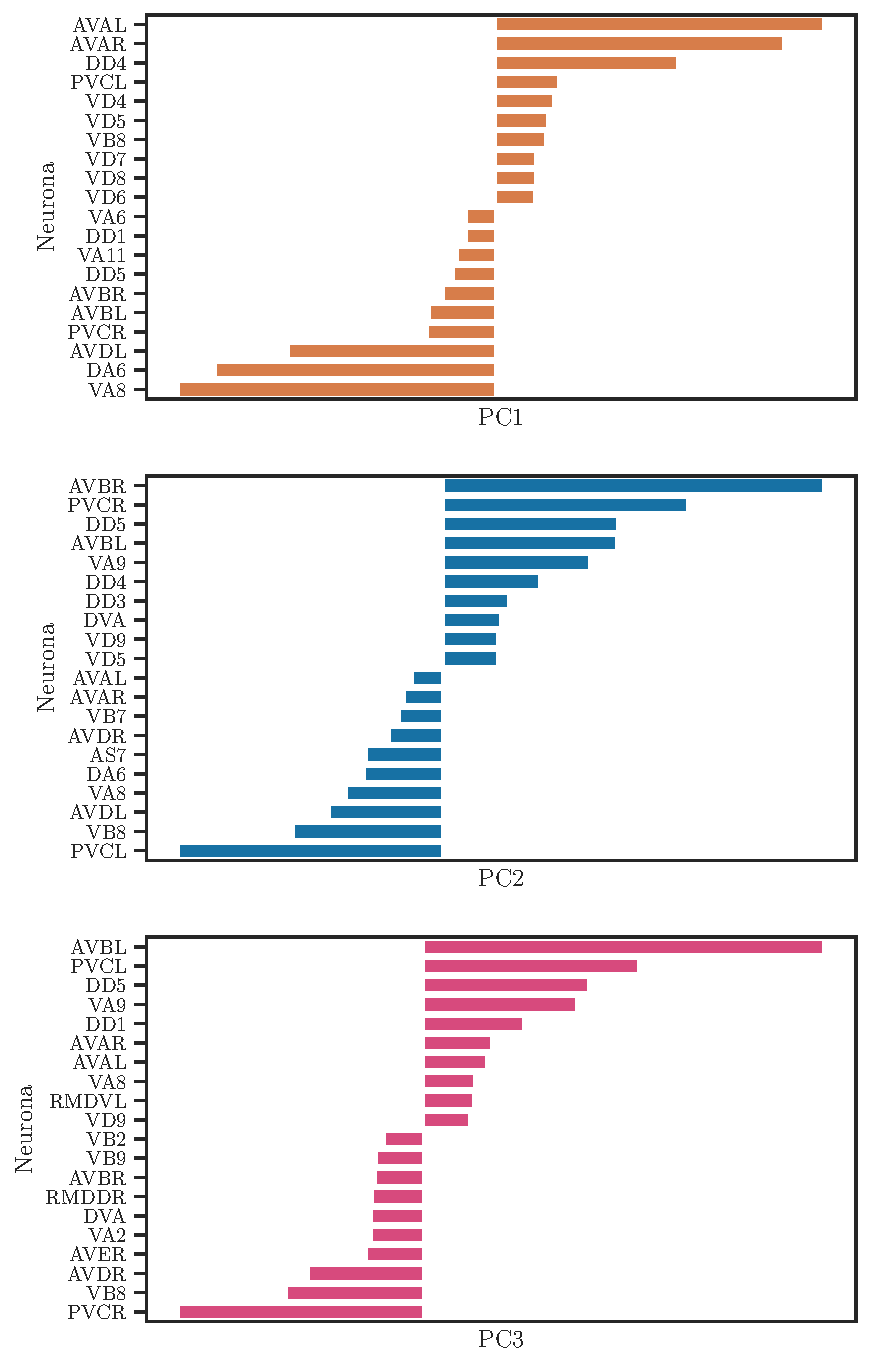
\includegraphics[width=\imsize]{PCs_robot.pdf}
 	\caption[Las neuronas están ordenas y agrupadas por sus pesos y signos de componentes principales (PC1-3).]{Las neuronas están ordenas y agrupadas por sus pesos y signos de componentes principales (PC1-3). (a) Coeficientes PC1, agrupados por orden de pesos. (b) Coeficientes PC2, (c) Coeficientes PC3.}\label{fig:pcs}
 \end{figure}


 \begin{figure}[h!]
	\centering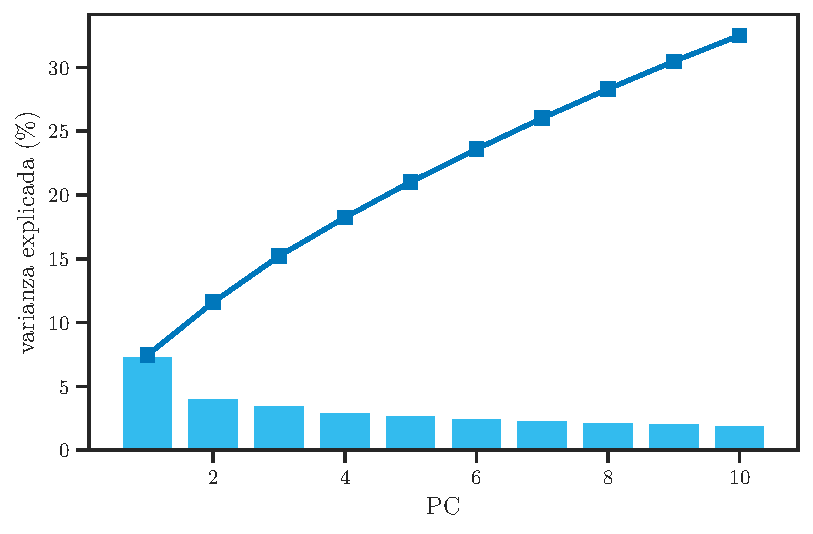
\includegraphics[width=\imsize]{varianza_explicada_robot.pdf}
	\caption[Varianza explicada por las primeros diez componentes principales, la línea azul oscuro indica la varianza acumulada explicada.]{Varianza explicada por las primeros diez componentes principales, la línea azul oscuro indica la varianza acumulada explicada.}\label{fig:varianza}
\end{figure}


La integral de tiempo del primer PC temporal mostró un patrón oscilatorio con variaciones en el tiempo, transiciones abruptas y períodos estables (\Cref{fig:ingegral_PCS}). Este patrón se deriva de la interacción entre dos grupos de interneuronas y neuronas motoras, previamente implicados en el control de la locomoción dirigida hacia adelante y hacia atrás. Notamos que las neuronas que anteriormente desempeñaban funciones opuestas tenían signos opuestos en sus pesos del primer PC (ver \Cref{fig:pcs} ; p. ej., AVA promueve el rastreo hacia atrás y AVB promueve el rastreo hacia adelante). En contraste, el segundo y tercer PC recibieron contribuciones significativas de las neuronas motoras de la cabeza, aunque sus pesos neuronales indicaron contribuciones de múltiples neuronas. Los patrones y contribuciones de los PC1 a PC3 se mantuvieron consistentes en múltiples repeticiones del experimento.


 \begin{figure}[h!]
	\centering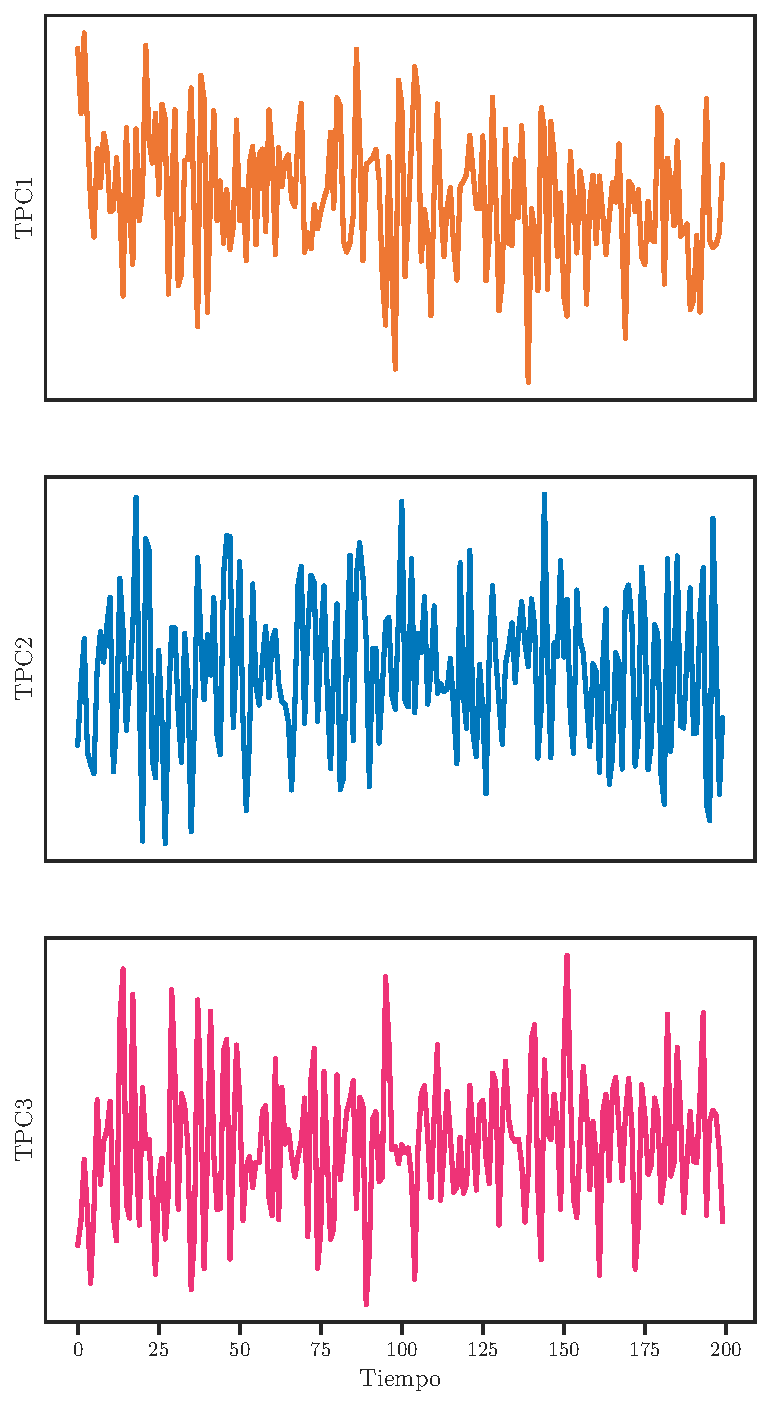
\includegraphics[width=\imsize]{TPCs_robot.pdf}
	\caption[ Integrales de los primeros tres PC temporales.]{ Integrales de los primeros tres PC temporales.}\label{fig:ingegral_PCS}
\end{figure}

El diagrama de fase de los PC1-3 (\Cref{fig:colector}) temporales mostró resultados similares a los de Kato et al. (\Cref{fig:kato}), en los que la evolución temporal del estado neural era cíclica, con estados que se repetían en cada ensayo. Estos ciclos de trayectoria formaban paquetes espacialmente coherentes en el espacio PCA. En consecuencia, toda la trayectoria del estado neural trazó un colector que definimos como el \textquote{subvolumen del espacio PCA ocupado por la trayectoria del estado neural}.  El hallazgo más destacado fue que, de manera similar a los resultados previos, la trayectoria del estado neural trazaba un conjunto que correspondía a diferentes comportamientos de locomoción. Estos comportamientos estaban asociados con la matriz de acciones realizadas por el robot (ver \Cref{fig:acciones}), donde cada trayectoria se relacionaba con una acción específica, representada por un color en nuestra visualización. Es importante destacar que las figuras anteriores se suavizaron mediante interpolación numérica. Nuestros resultados sugieren que la dinámica neural puede ser utilizada para predecir el comportamiento de un gusano C. elegans. Esto abre nuevas posibilidades para el desarrollo de robots bioinspirados que imitan el comportamiento de los animales.


 \begin{figure}[h!]
	\centering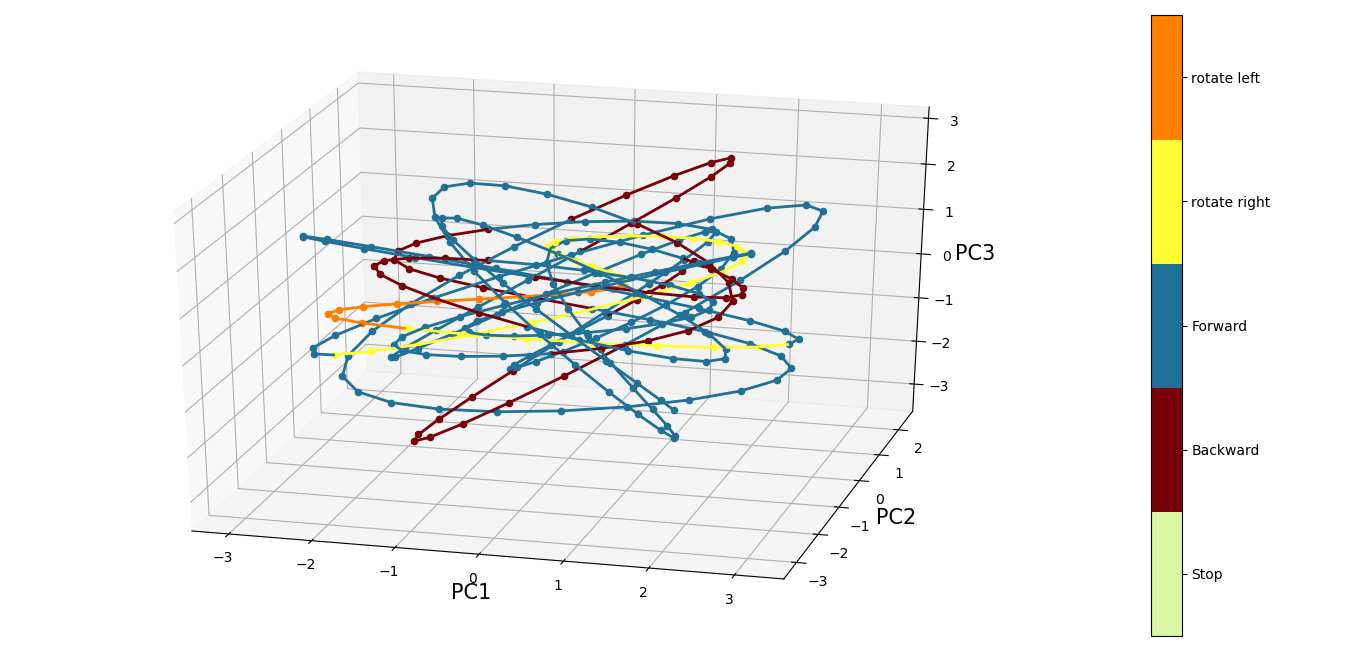
\includegraphics[width=\imsize]{PCs.png}
	\caption[ Dinámica neural global y acciones. Diagramas de fase de los tres primeros PC temporales en un intervalo de tiempo seleccionado.  ]{Dinámica neural global y acciones. Diagramas de fase de los tres primeros PC temporales en un intervalo de tiempo seleccionado. Las acciones del robot se representan con diferentes colores. La figura muestra que la dinámica global evoluciona en una órbita similar a un atractor de baja dimensión, donde diferentes segmentos de la trayectoria corresponden a estados motores bien definidos.}\label{fig:colector}
\end{figure}


 \begin{figure}[h!]
	\centering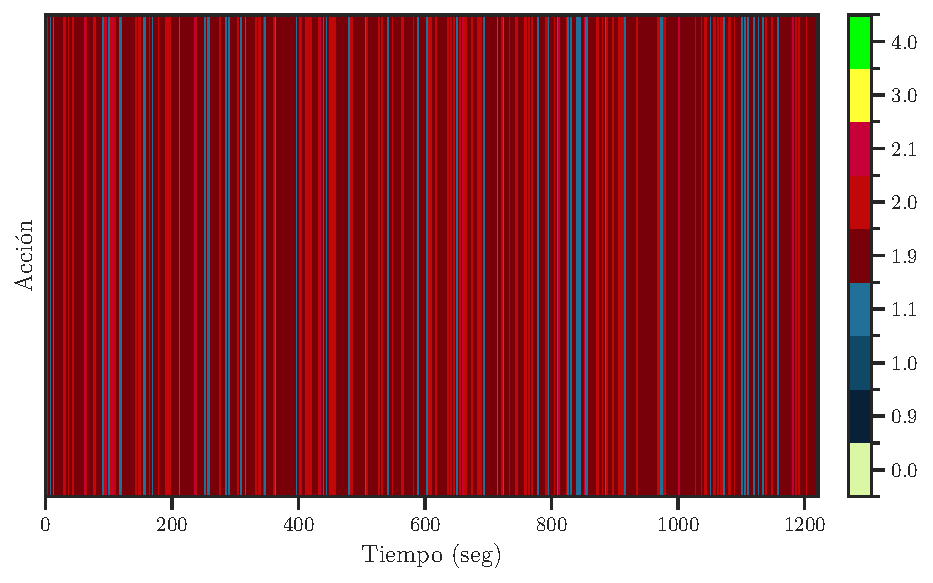
\includegraphics[width=\imsize]{accion_robot.pdf}
	\caption[ Matriz de acciones realizadas por el robot]{Matriz de acciones realizadas por el robot.}\label{fig:acciones}
\end{figure}


 \begin{figure}[h!]
	\centering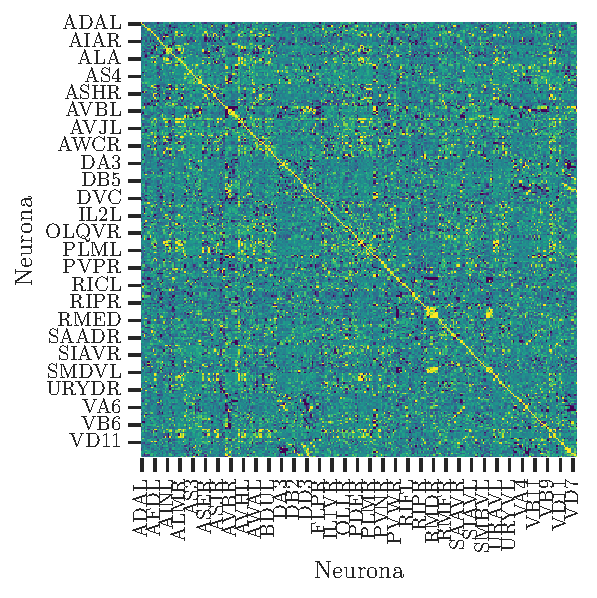
\includegraphics[width=\imsize]{correlacion_robot.pdf}
	\caption[ Correlación de Activación entre Neuronas.]{Correlación de Activación entre Neuronas.  En amarillo, se resaltan las neuronas que presentan correlación significativa, indicando que la dinámica global del robot se organiza en grupos o clústeres de neuronas. Esto sugiere una actividad de red rica y coordinada.}\label{fig:correlacion_robot}
\end{figure}

\subsection{Discusión}

Esta sección se centro en  la dinámica global y su relación con la acción. Al igual que \cite{kato_global_2015}, construimos series temporales de PC temporales tomando promedios ponderados de cada componente principal con la serie temporal mulineuronal completa. Esto permite una reducción drástica de la dimensionalidad, donde las PC temporales tienen señales que son representativas de grupos neuronales. La \Cref{fig:correlacion_robot} muestra un mapa de calor que representa la correlación de activación entre las neuronas en el robot. Las áreas coloreadas en amarillo indican que ciertas neuronas están correlacionadas, lo que sugiere una organización en grupos o clústeres de neuronas en la dinámica del robot. Esta correlación de actividad neuronal resalta la existencia de una red neuronal rica y coordinada en el sistema, lo que puede tener implicaciones significativas en la generación de comportamientos emergentes y adaptativos en el robot.

En la \Cref{fig:colector}  mostramos una representación paramétrica de las integrales temporales de las tres primeras PC temporales en un intervalo de tiempo fijo. La trayectoria presenta un comportamiento similar al de un sistema dinámico en una órbita tipo atractor. Además, encontramos que las trayectorias de la serie temporal completa de los experimentos siempre presentaban este comportamiento, y permanecían acotadas en un estado global caracterizado por la presencia de órbitas cíclicas.

Cuando se tuvo en cuenta la actividad del robot, encontramos que diferentes segmentos de las trayectorias corresponden a diferentes acciones. Esto se puede ver claramente en la \Cref{fig:colector}, donde utilizamos diferentes colores para representar la acción que el robot estaba ejecutando en un momento dado. Elegimos un segmento de tiempo particular en el que el robot se encuentra con un obstáculo, se detiene, retrocede y giraba. Obsérvese que las diferentes acciones pueden distinguirse claramente como segmentos bien definidos de la trayectoria.

En C. elegans, Kato et al. \cite{kato_global_2015} encontraron que la actividad neuronal evoluciona en una variedad de baja dimensión similar a un atractor. Además, diferentes segmentos en esta variedad, que corresponden a la sincronización de diferentes grupos de neuronas, están claramente correlacionados con diferentes estados motores. Nuestros resultados destacan el papel que juega el connectoma en la emergencia de estos estados cíclicos tipo atractor.




\section{Dinámicas neuronales emergentes}

 \subsection{ Sincronización de frecuencia y fase}

En este apartado analizaremos la correlación entre la dinámica global y el conectoma subyacente. Vale la pena destacar que en el modelo robótico, todas las neuronas tienen el mismo umbral de disparo y, por lo tanto, tienen dinámicas individuales idénticas como unidades aisladas. Sin embargo, esperamos que sus dinámicas reflejen la distribución no uniforme de la conectividad sináptica. Por ejemplo, las neuronas en una posición central, con un gran número de entradas o conexiones con pesos grandes, pueden alcanzar el umbral más rápido y, por lo tanto, disparar con frecuencia. De hecho, descubrimos que AVAL, AVBR y AVBL, nodos con la mayor centralidad de grado y también con la mayor centralidad de cercanía \cite{varshney_structural_2011}, oscilan con alta frecuencia. En contraste, los nodos en una posición periférica reciben menos entradas y, por lo tanto, tardarán más en alcanzar el umbral, lo que conduce a una dinámica más lenta. En la \Cref{fig:sincronia_1}A representamos las señales de tres neuronas motoras del cordón ventral en un intervalo de tiempo fijo, mostrando oscilaciones a diferentes frecuencias. Caracterizamos cuantitativamente estas oscilaciones realizando una transformada de Fourier (FT; \Cref{fig:sincronia_1}B). Encontramos que el valor real de la FT presenta picos definidos y, por lo tanto, definimos la frecuencia característica de las neuronas, $\Omega$, como el pico más alto en la FT.


 \begin{figure}[h!]
	\centering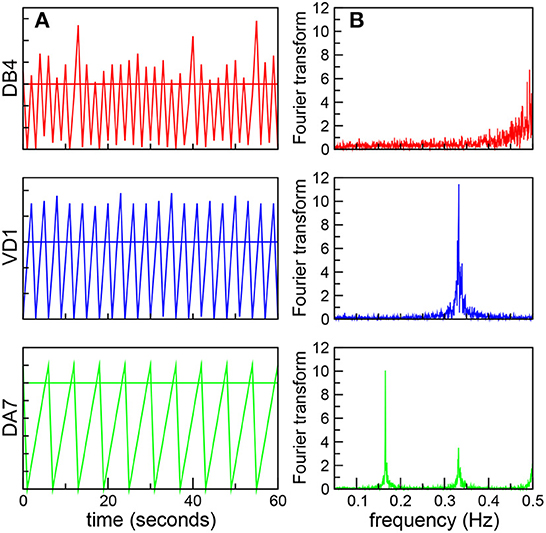
\includegraphics[width=\imsize]{sincronia1.jpg}
	\caption[ Las neuronas oscilan a diferentes frecuencias.]{Las neuronas oscilan a diferentes frecuencias. (A) Dinámica de tres neuronas motoras del cordón ventral, DB4 (arriba, rojo), VD1 (medio, azul) y DA7 (abajo, verde). La figura muestra las señales neuronales en función del tiempo en el mismo intervalo de tiempo de 60 segundos. Las líneas horizontales muestran el valor umbral h = 30. (B) Transformadas de Fourier correspondientes con picos definidos, utilizados para definir la frecuencia característica $\Omega$.}\label{fig:sincronia_1}
\end{figure}

Como se discutió en el \Cref{sec:kato}  Kato et al.\cite{kato_global_2015} registraron experimentalmente grupos de neuronas que presentan dinámicas coordinadas en C. elegans.  Con esta idea en mente, cuando extendemos nuestro enfoque de la dinámica individual a la colectiva, observamos que algunas neuronas se agrupan en grupos que comparten la misma frecuencia característica. Incluso más, en algunos casos la forma completa de su transformada de Fourier (FT), incluidos los picos más pequeños, se superpone. Esto nos permite definir grupos sincronizados como grupos de neuronas con FTs superpuestas.

 \begin{figure}[h!]
	\centering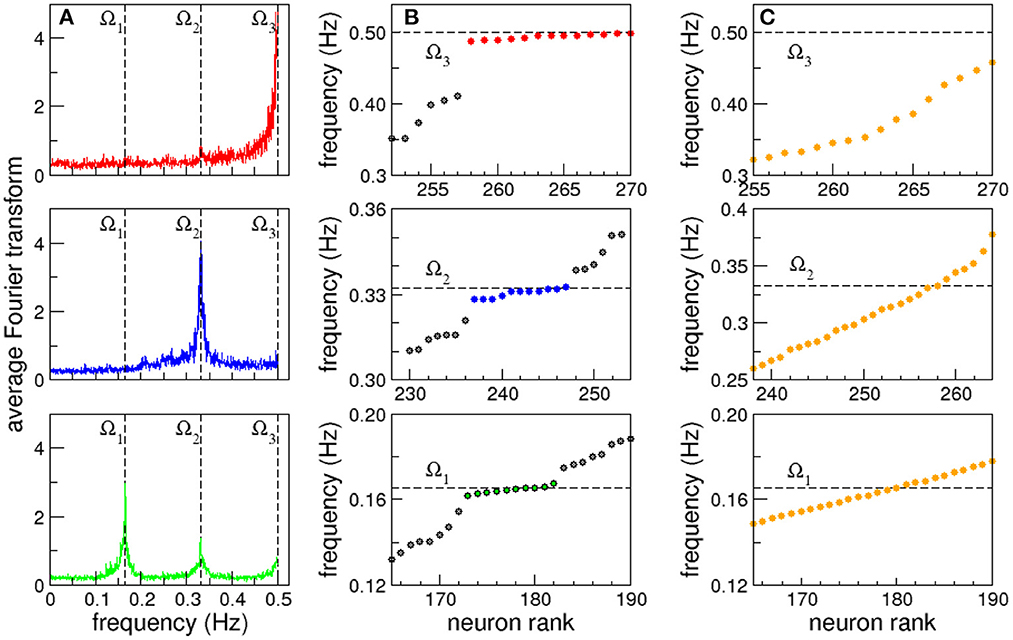
\includegraphics[width=\imsize]{sincronia2.jpg}
	\caption[ Sincronización de frecuencias.]{Sincronización de frecuencias. (A) Transformadas de Fourier promedio de las neuronas en tres grupos sincronizados para un experimento completo de 15 minutos de duración. (B) Neuronas ordenadas de menor a mayor frecuencia característica. Las líneas discontinuas se muestran como una guía para el ojo para mostrar la frecuencia característica de los grupos sincronizados que aparecen como líneas horizontales. (C) No se observan grupos sincronizados en los experimentos de control con versiones aleatorias del  conectoma.}\label{fig:sincronia_2}
\end{figure}

En la \Cref{fig:sincronia_2}A, trazamos la transformada de Fourier promedio de las neuronas en tres grupos sincronizados de frecuencia diferente. Las transformadas de Fourier promediadas tienen picos agudos, que nos permiten definir los grupos $\Omega$ por su frecuencia característica (media $\pm$ desviación estándar): $\Omega_1 = 0.165 \pm 0.002$ Hz (verde, inferior), $\Omega_2 = 0.332 \pm 0.003$ Hz (azul, medio) y $\Omega_3 = 0.496 \pm 0.004$ Hz (rojo, superior; consulte también las  \Cref{table:cluster_1,table:cluster_2,table:cluster_3} y las \Cref{fig:cluster_1,fig:cluster_2,fig:cluster_3} para una lista completa de neuronas en cada grupo, sus señales individuales y las FT correspondientes). Tenga en cuenta que $\Omega_2$ y $\Omega_3$ son aproximadamente múltiplos enteros de $\Omega_1$. Si bien el origen de tal relación armónica aparente aún no está claro, tener solo tres frecuencias no puede excluirse una coincidencia aleatoria. La \Cref{fig:sincronia_2}B muestra en detalle los tres grupos sincronizados cuando las neuronas se ordenan de menor a mayor frecuencia característica. Usamos líneas discontinuas como una guía para el ojo para mostrar las frecuencias características $\Omega$ de los grupos sincronizados que aparecen como líneas horizontales. En este punto, vale la pena enfatizar que la aparición de grupos sincronizados no parece depender de la topografía particular donde se mueve el robot. Esto se debe al hecho de que las neuronas sensoriales asociadas con el comportamiento de evitación solo se estimulan cuando el sensor de distancia mide una distancia por debajo del umbral y, dado que entonces el robot responde retrocediendo, el intervalo de tiempo en el que las neuronas sensoriales son estimuladas suele ser muy corto. Como consecuencia, la dinámica neuronal global converge rápidamente de nuevo a un atractor global.


 \begin{table}[h!]
	\centering
	\caption[La tabla  presenta las neuronas del grupo sincronizado $\Omega_1$, su descripción, la frecuencia característica correspondiente y el peso del primer componente principal (PC1). ]{ La tabla  presenta las neuronas del grupo sincronizado $\Omega_1$, su descripción, la frecuencia característica correspondiente y el peso del primer componente principal (PC1).  VCMN = Neurona motora del cordón ventral, 
		RVCI = Neurona interneuronal del anillo y el cordón ventral, RI = Neurona interneuronal del anillo.}
	\begin{tblr}{colspec={llll},
			row{odd} = {bg=gray8},
			row{even} = {bg=gray9},
			row{1} = {bg=red3, fg=white, font=\sffamily},
		}
		
Neurona & Descripción & $\Omega$  & PC1 \\
DA7  &  VCMN &  $0.166 \pm 0.001$ & $2.7 \pm 0.1$ \\
AVL  & RVCI & $0.164 \pm 0.001$ & $1.6 \pm 0.1$ \\
AS2 & VCMN & $0.163 \pm 0.001$ &  $0.1 \pm 0.1$ \\
DB4  & VCMN &  $0.165 \pm 0.001$ & $0.1 \pm 0.1$ \\
RMDL & VCMN & $0.167 \pm 0.001$ & $-0.2 \pm 0.1$ \\
VA7 & VCMN & $0.166 \pm 0.001$ & $-0.8 \pm 0.1$ \\
DD6 & VCMN & $0.166 \pm 0.001$ & $-1.2 \pm 0.1$ \\
SABVR & RI &  $0.162 \pm 0.001$ & $-4.2 \pm 0.1$\\
RID & RI & $0.164 \pm 0.001$ & $-7.1 \pm 0.1$\\
VD7 & VCMN & $0.165 \pm 0.001$ &  $-13.5 \pm 0.1$
	\end{tblr}
	\label{table:cluster_1}
\end{table}



\begin{table}[h!]
	\centering
	\caption[La tabla  presenta las neuronas del grupo sincronizado $\Omega_2$, su descripción, la frecuencia característica correspondiente y el peso del primer componente principal (PC1). ]{ La tabla  presenta las neuronas del grupo sincronizado $\Omega_2$, su descripción, la frecuencia característica correspondiente y el peso del primer componente principal (PC1).  VCMN = Neurona motora del cordón ventral}
	\begin{tblr}{colspec={llll},
			row{odd} = {bg=gray8},
			row{even} = {bg=gray9},
			row{1} = {bg=red3, fg=white, font=\sffamily},
		}
		
		Neurona & Descripción & $\Omega$  & PC1 \\
		VA11  &  VCMN &  $0.331 \pm 0.001$ & $15.3 \pm 0.1$ \\
		VA6  & VCMN & $0.331 \pm 0.001$ &  $9.8 \pm 0.1$ \\
		DA5 & VCMN &  $0.333 \pm 0.001$ &  $7.4 \pm 0.1$ \\
		VD3 & VCMN & $0.328 \pm 0.001$ &  $3.9 \pm 0.1$\\
		VD1  & VCMN& $0.330 \pm 0.001$ &  $0.6 \pm 0.1$ \\
		DA1 & VCMN & $0.332 \pm 0.001$ &  $-1.7 \pm 0.1$ \\
		AS11 & VCMN & $0.328 \pm 0.001$ & $-2.5 \pm 0.1$ \\
		DD3 & VCMN & $0.331 \pm 0.001$ &  $-6.4 \pm 0.1$ \\
		VD4 & VCMN & $0.328 \pm 0.001$ &  $-7.1 \pm 0.1$\\
		VD6 & VCMN &  $0.332 \pm 0.001$ &  $-12.7 \pm 0.1$\\	
		
	\end{tblr}
	\label{table:cluster_2}
\end{table}


\begin{table}[h!]
	\centering
	\caption[La tabla  presenta las neuronas del grupo sincronizado $\Omega_3$, su descripción, la frecuencia característica correspondiente y el peso del primer componente principal (PC1). ]{ La tabla  presenta las neuronas del grupo sincronizado $\Omega_3$, su descripción, la frecuencia característica correspondiente y el peso del primer componente principal (PC1).  VCMN = Neurona motora del cordón ventral, Interneurona del cordón ventral.}
	\begin{tblr}{colspec={llll},
			row{odd} = {bg=gray8},
			row{even} = {bg=gray9},
			row{1} = {bg=red3, fg=white, font=\sffamily},
		}
		
		Neurona & Descripción & $\Omega$  & PC1 \\
       VA8 & VCMN & $0.498 \pm 0.001$ & $110.1 \pm 0.1$\\
       DA6  & VCMN & $0.496 \pm 0.001$ & $95.8 \pm 0.1$\\
       AVDL & VCI & $0.496 \pm 0.001$ & $76.1 \pm 0.1$\\
       AS7 & VCMN  & $0.495 \pm 0.001$ & $29.9 \pm 0.1$\\
       AS8 & VCMN & $0.496 \pm 0.001$ & $17.8 \pm 0.1$\\
       AS9 & VCMN & $0.491 \pm 0.001$ & $5.7 \pm 0.1$\\
       PVCR & VCI  & $0.488 \pm 0.001$ &  $15.1 \pm 0.1$\\
       AVBL & VCI  & $0.499 \pm 0.001$ & $-10.1 \pm 0.1$ \\
       DD4 & VCMN & $0.499 \pm 0.001$ &  $-51.2 \pm 0.1$\\
       AVAR & VCI & $0.489 \pm 0.001$ & $-84.9 \pm 0.1$\\
       AVAL & VCI & $0.499 \pm 0.001$ & $-99.8 \pm  0.1$
		
	\end{tblr}
	\label{table:cluster_3}
\end{table}

 \begin{figure}[h!]
	\centering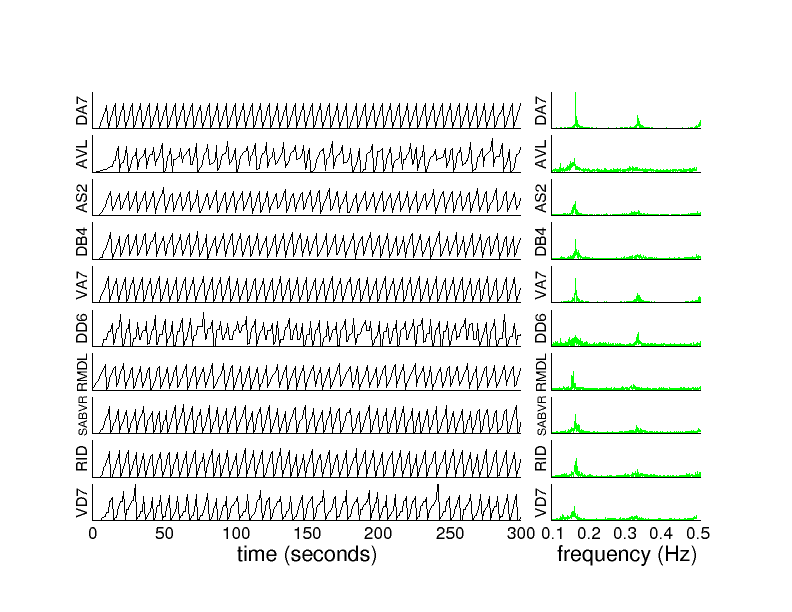
\includegraphics[width=\imsize]{cluster1.png}
	\caption[ Señales de todas las neuronas del grupo sincronizado $\Omega_1$ en un intervalo de cinco minutos, y sus transformadas de Fourier correspondientes en un experimento de 20 minutos de duración.]{Señales de todas las neuronas del grupo sincronizado $\Omega_1$ en un intervalo de cinco minutos, y sus transformadas de Fourier correspondientes en un experimento de 20 minutos de duración.}\label{fig:cluster_1}
\end{figure}
 \begin{figure}[h!]
	\centering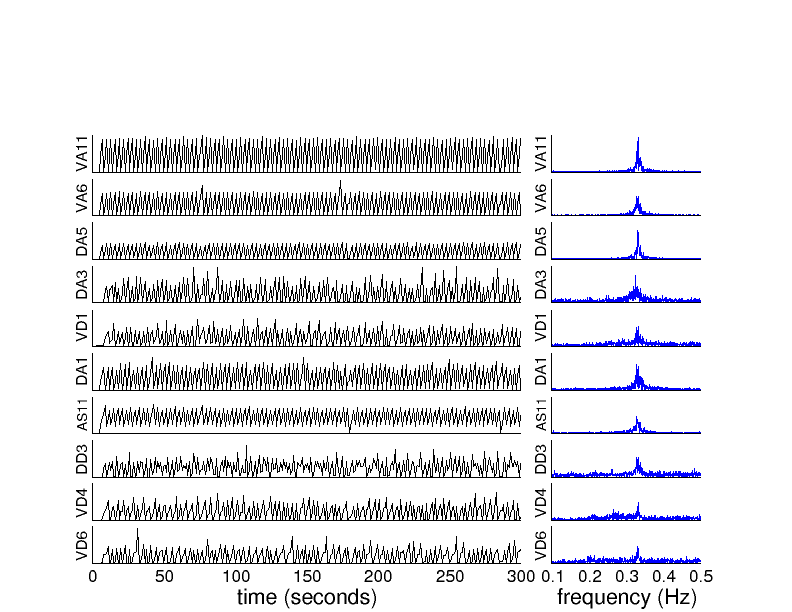
\includegraphics[width=\imsize]{cluster_2.png}
	\caption[ Señales de todas las neuronas del grupo sincronizado $\Omega_2$ en un intervalo de cinco minutos, y sus transformadas de Fourier correspondientes en un experimento de 20 minutos de duración.]{Señales de todas las neuronas del grupo sincronizado $\Omega_1$ en un intervalo de cinco minutos, y sus transformadas de Fourier correspondientes en un experimento de 20 minutos de duración.}\label{fig:cluster_2}
\end{figure}
 \begin{figure}[h!]
	\centering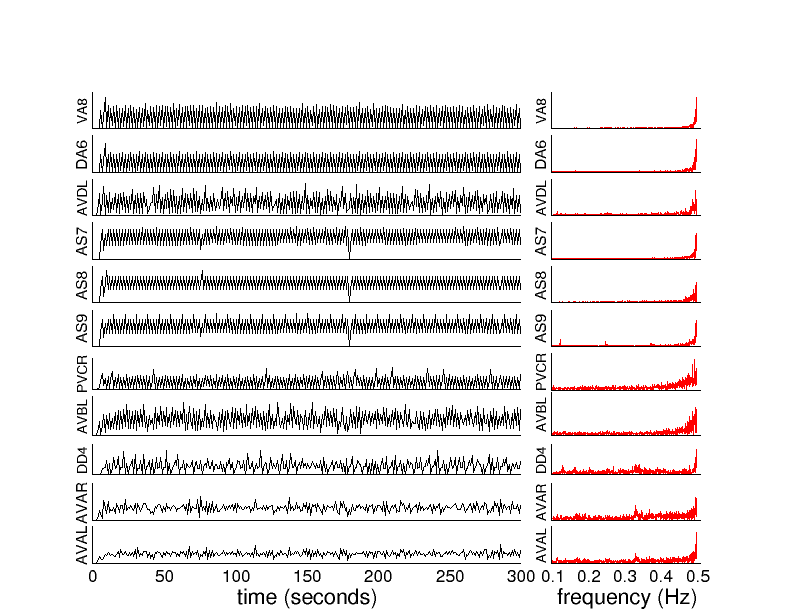
\includegraphics[width=\imsize]{cluster_3.png}
	\caption[ Señales de todas las neuronas del grupo sincronizado $\Omega_3$ en un intervalo de cinco minutos, y sus transformadas de Fourier correspondientes en un experimento de 20 minutos de duración.]{Señales de todas las neuronas del grupo sincronizado $\Omega_1$ en un intervalo de cinco minutos, y sus transformadas de Fourier correspondientes en un experimento de 20 minutos de duración.}\label{fig:cluster_3}
\end{figure}

La \Cref{fig:sincronia_2}B se asemeja mucho a la formación de grupos sincronizados en osciladores Kuramoto con una amplia distribución de frecuencias naturales \cite{manrubia_emergence_2004}.  Sin embargo, en este caso, los nodos tienen una dinámica idéntica, ya que todas las neuronas tienen el mismo umbral de disparo, y la heterogeneidad surge de la compleja red de interacciones dada por el conectoma de C. elegans. Una comparación directa de la lista de entradas sensoriales y salidas cinéticas con las neuronas de los grupos sincronizados revela que no es un efecto trivial de la estimulación directa (Ver la \Cref{sec:dinamica} para ver las neuronas estimuladas).  Como se discutió en el \Cref{sec:aleaotrioconectoma} para probar que la emergencia de grupos sincronizados no es un epifenómeno, analizamos la dinámica en versiones aleatorizadas del conectoma donde se conservan la distribución de grados y las distribuciones de pesos. Es decir, las redes aleatorias tienen exactamente la misma distribución de grados de entrada y salida y distribuciones de pesos asignadas aleatoriamente a los nodos y enlaces. En todos los casos, encontramos que las acciones emergentes del robot se pierden (ver video suplementario S2) y no se observan grupos sincronizados (ver \Cref{fig:sincronia_2}C).

Como se discutió anteriormente Kato et al. \cite{kato_global_2015} utilizaron técnicas de imagen de calcio para registrar la actividad neuronal con resolución de célula única en todos los ganglios cefálicos y algunas neuronas motoras del cordón ventral. En estos experimentos, se escanearon $\sim$100 neuronas tres veces por segundo durante periodos de 20 minutos, generando conjuntos de datos de alta dimensión. Utilizando el análisis de componentes principales (PCA) para la reducción de dimensionalidad, pudieron agrupar neuronas con señales correlacionadas. En particular, produjeron vectores de pesos neuronales (PC), mostrando que los grupos con signos opuestos en sus PC oscilan en antifase, y que de acuerdo con el signo de su vector de pesos se correlacionan con el comportamiento hacia adelante o hacia atrás del gusano.   Siguiendo el mismo procedimiento, también realizamos un análisis de componentes principales similar. Al igual que en Kato et al., cada una de las series temporales neuronales se normalizó utilizando el valor medio ($\bar{s}$) y la desviación estándar ($\sigma_s$):

\begin{equation}
s^{\prime}(t)=\frac{s(t)-\bar{s}(t)}{\sigma_s(t)}
\end{equation}


de modo que las nuevas series temporales tienen ahora media cero y desviación estándar unitaria. A continuación, se calcularon los componentes principales en función de la estructura de covarianza de los datos normalizados, produciendo vectores de pesos neuronales (PC) para las series temporales neuronales de todas las neuronas del robot. Esto nos permitió avanzar en la caracterización cuantitativa de los grupos sincronizados en frecuencia.  En la \Cref{fig:sincronia_3} (arriba) representamos las frecuencias características de los tres grupos sincronizados en frecuencia $\Omega_1$ (verde), $\Omega_2$ (azul) y $\Omega_3$ (rojo) ya presentados en la \Cref{fig:sincronia_2}. Las neuronas se han ordenado ahora en función de su primer peso de componente principal (PC1; \Cref{fig:sincronia_3} (abajo)), es decir, las neuronas de la izquierda tienen el valor positivo más alto, mientras que las de la derecha tienen el valor negativo más bajo de PC1. Obsérvese que todos los grupos sincronizados implican neuronas con valores de PC1 tanto positivos como negativos. El grupo con menor frecuencia, $\omega_1$, presenta una amplia distribución de pesos neuronales. Para frecuencias más altas, las neuronas presentan una mayor segregación hacia valores extremos de PC1. De hecho, tanto $\Omega_2$ como $\Omega_3$ están claramente divididos en dos subgrupos más pequeños: uno con solo valores positivos de PC1 y otro con solo valores negativos de PC1. Esta segregación refleja diferencias en los tiempos de disparo de las neuronas. En cada grupo, los tiempos de disparo de las neuronas son proximales. En cambio, cuando se comparan las señales de las neuronas entre grupos, se observa un desplazamiento en su fase relativa. El mayor desplazamiento se produce para valores extremos de PC, cuando las neuronas de los diferentes subgrupos de la misma frecuencia oscilan principalmente en antifase (véase la \Cref{fig:antifase}).

 \begin{figure}[h!]
	\centering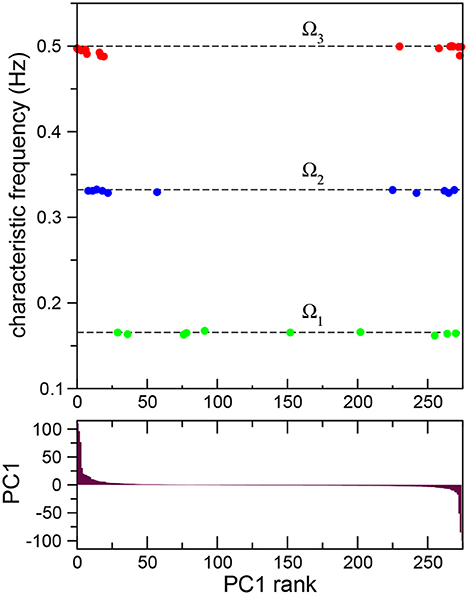
\includegraphics[width=\imsize]{sincronia3.jpg}
	\caption[ Sincronización de frecuencias ordenada según el análisis de componentes principales.]{Sincronización de frecuencias ordenada según el análisis de componentes principales. Transformadas de Fourier promedio de las neuronas de tres grupos sincronizados en frecuencia (arriba) para un experimento completo de 15 minutos de duración ordenadas según su primer componente principal PC1 (abajo). El análisis revela la presencia de subgrupos con signos opuestos en su peso de componente principal.}\label{fig:sincronia_3}
\end{figure}

 \begin{figure}[h!]
	\centering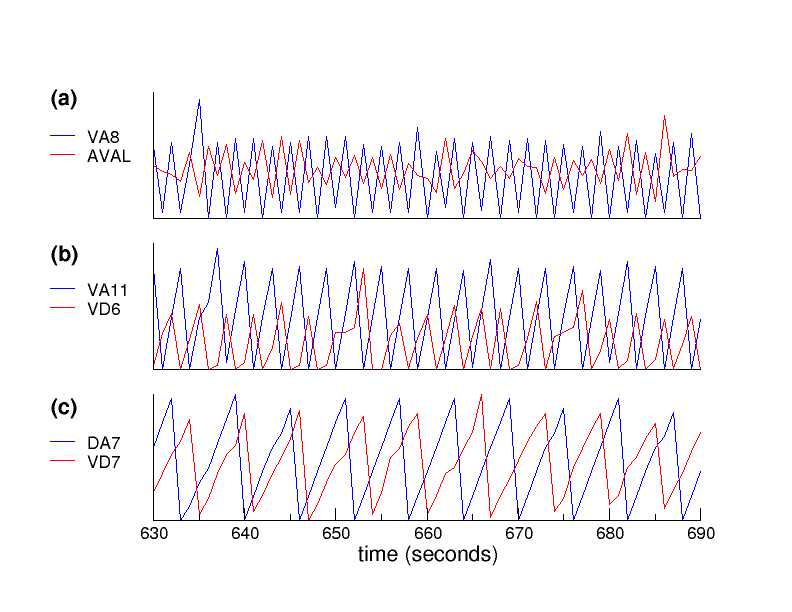
\includegraphics[width=\imsize]{antifase.png}
	\caption[ Sincronización de frecuencias ordenada según el análisis de componentes principales.]{Oscilaciones en antifase de las neuronas con el mayor PC1 positivo (azul) y el menor PC1 negativo (rojo). (a) VA8 y AVAL en el grupo $\Omega_3$, (b) VA11 y VD6 en el grupo $\Omega_2$, y (c) DA7 y VD7 en el grupo $\Omega_1$. Todas las figuras se presentan en el mismo intervalo de tiempo de 60 segundos.}\label{fig:antifase}
\end{figure}

\subsection{Dinámica neuronal anidada}

Ahora analizamos cómo las oscilaciones colectivas en los grupos sincronizados en frecuencia también están acopladas entre sí. En la \Cref{fig:sincronia_2}A mostramos las transformadas de Fourier promedio de las neuronas en tres grupos sincronizados en frecuencia. Obsérvese que la TF promedio del grupo con la frecuencia más baja, $\Omega_1$, también tiene dos picos más pequeños, que coinciden con la frecuencia característica de los otros grupos: $\Omega_2$ y $\Omega_3$. Como guía para el ojo, indicamos con líneas discontinuas estas frecuencias en los tres paneles. Esto revela un acoplamiento entre los diferentes grupos sincronizados en frecuencia.

Para estudiar cuantitativamente el acoplamiento entre oscilaciones a diferentes frecuencias, analizamos las señales de las neuronas de un grupo dado cuando la señal de una neurona de otro grupo con una frecuencia característica más baja alcanza su máximo \cite{jensen_cross-frequency_2007}.   Si hay un acoplamiento entre las oscilaciones, entonces esperamos que la señal de la neurona con mayor frecuencia pueda presentar pequeñas fluctuaciones alrededor del mismo valor medio cada vez que se alcanza el máximo con la frecuencia más baja. Por el contrario, si no hay acoplamiento, se espera que la señal varíe aleatoriamente. En la \Cref{fig:anidado} representamos las señales de las neuronas de $\Omega_2$ y $\Omega_3$ cuando una neurona seleccionada del grupo con menor frecuencia característica $\Omega_1$ alcanza su máximo. En particular, nos centramos en las neuronas con el mayor peso de PC1 positivo en cada uno de los grupos sincronizados. Las Figuras \Cref{fig:anidado}A, B muestran que estas neuronas están acopladas, ya que el mismo valor medio persiste en intervalos de tiempo prolongados. Además, para visualizar este resultado, representamos en la \Cref{fig:anidado}E las señales de estas neuronas en un intervalo de tiempo fijo, utilizando líneas verticales discontinuas como guía para el ojo. La figura muestra claramente una relación jerárquica anidada entre oscilaciones a diferentes frecuencias. En las \Cref{fig:anidado}C, D representamos las señales de las neuronas que tienen los pesos de PC1 negativos más bajos. En marcado contraste con las neuronas con pesos positivos, las señales no están correlacionadas y fluctúan a lo largo de todo el experimento.


 \begin{figure}[h!]
	\centering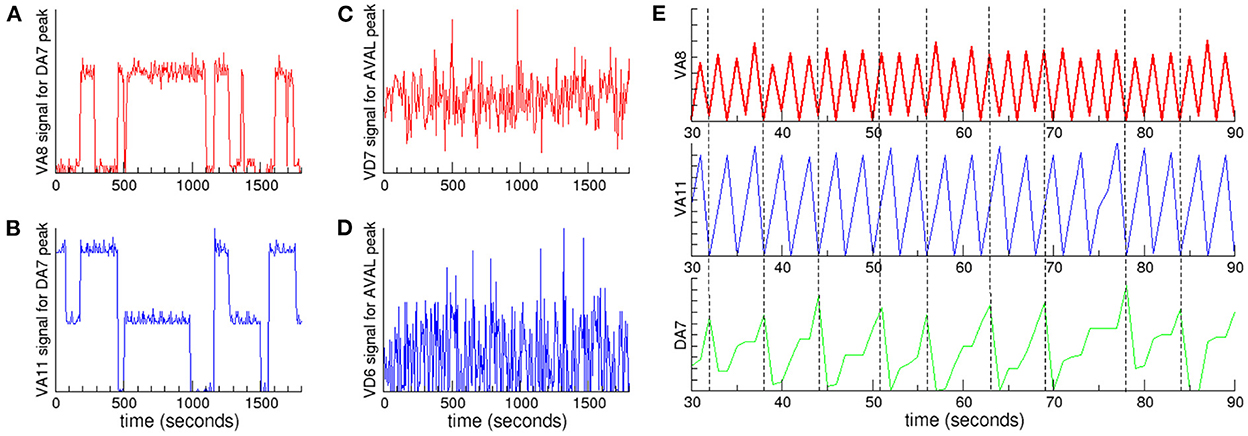
\includegraphics[width=\imsize]{anidado.jpg}
	\caption[ Dinámica neuronal anidada.]{Dinámica neuronal anidada. Representamos las señales de las neuronas de los grupos $\Omega_2$ y $\Omega_3$ cuando una neurona seleccionada del grupo $\Omega_1$ alcanza su máximo: (A) señal de VA8 (roja) del grupo $\Omega_3$ y (B) VA11 (azul) del grupo $\Omega_2$, cuando DA7 del grupo $\Omega_1$ alcanza su máximo. El acoplamiento entre las neuronas de estos grupos aparece como regiones caracterizadas por señales con pequeñas fluctuaciones alrededor de un valor medio. En cambio, cuando no hay acoplamiento las señales presentan grandes fluctuaciones, como se muestra por ejemplo para las señales de (C) VD7 (roja) del grupo $\Omega_3$ y (D) VD6 (azul) del grupo $\Omega_2$, cuando AVAL del grupo $\Omega_1$ alcanza su máximo. (E) Un intervalo de tiempo de 60 segundos de los datos presentados en (A, B) muestra la relación jerárquica. Las señales corresponden a VA8 (roja), VA11 (azul) y DA7 (verde). Las líneas verticales discontinuas son una guía para el ojo que muestran el momento en que DA7 alcanza su máximo.}\label{fig:anidado}
\end{figure}

\subsection{Dinámica neuronal y acciones del robot}

En esta sección analizamos la correlación entre la dinámica neuronal emergente y las acciones del robot. El modelo robótico es muy adecuado para este estudio, ya que permite registrar la dinámica neuronal mientras se registran simultáneamente las acciones. Para determinar si había una correlación entre una acción determinada y la actividad de neuronas específicas, contrastamos las series temporales de la dinámica neuronal con las series temporales de las acciones del robot. En primer lugar, registramos todos los eventos de acción en un experimento de 20 minutos de duración. A continuación, analizamos qué acciones estaba ejecutando el robot cuando una neurona determinada se había activado, es decir, cuando su valor se restablecía a cero. Por último, contrastamos las fracciones de eventos de estas dos series temporales para ver si había variaciones significativas.

En los experimentos, el robot se mueve principalmente hacia adelante y hacia atrás, mientras que los giros suelen ser eventos cortos en los que el robot solo cambia de dirección, por lo que nos centramos principalmente en los eventos de avance y retroceso. Estos eventos corresponden a la respuesta de la red a la estimulación de las neuronas sensoriales \footnote{\url{https://wormatlas.org/hermaphrodite/nervous/Images/neurotable1leg.htm}}.  Como se discutió en el \Cref{sec:estimuladas}  tal como se observa en el gusano, la estimulación de las neuronas de quimiotaxis promueve el desplazamiento sostenido y hace que el robot se mueva hacia adelante, mientras que la estimulación de las neuronas sensoriales que promueven la evitación hace que el robot se mueva hacia atrás. En este punto, cabe destacar que estas respuestas de acción son emergentes y no triviales, en el sentido de que solo se estimula una pequeña fracción de todas las unidades dinámicas, y por lo tanto las respuestas corresponden a una modulación de la dinámica global.


Encontramos que las neuronas de los grupos sincronizados con los mayores pesos de PC1 positivos promueven eventos de avance, mientras que las neuronas con los pesos negativos más bajos promueven eventos de retroceso. La \Cref{fig:neuronas_comportamiento} muestra la fracción de eventos registrados cuando se disparan las neuronas con los mayores pesos de PC1 positivos y negativos en los grupos sincronizados (véase también el \Cref{table:neuronas_comportamiento}). Las barras de color corresponden a: $\Omega_1$ (verde), $\Omega_2$ (azul) y $\Omega_3$ (rojo). En cada figura, los resultados se contrastan con las fracciones de eventos para todo el experimento (barras grises). Obsérvese que se observa un aumento significativo de los eventos de avance cuando se disparan las neuronas con el mayor PC1 positivo (primeras columnas de las \Cref{fig:neuronas_comportamiento}A, C, E), mientras que se observa una reducción en las neuronas con el menor PC1 negativo (primeras columnas de las \Cref{fig:neuronas_comportamiento}B, D, F). Al mismo tiempo, se observa un aumento de los eventos de retroceso cuando se disparan neuronas con PC negativas (columnas discontinuas de las \Cref{fig:neuronas_comportamiento}B, D, F), mientras que se observa una disminución de la fracción de eventos de retroceso en las neuronas con pesos positivos (columnas discontinuas de las \Cref{fig:neuronas_comportamiento}A, C, E). Estos resultados revelan el papel que juega la segregación de las neuronas en los grupos sincronizados en la promoción de diferentes acciones que el robot ejecuta. Es interesante que, en C. elegans, Kato et al. \cite{kato_global_2015} observaron que las neuronas que promueven comportamientos opuestos, como el avance y el retroceso, también tienen signos opuestos en sus pesos de PC1.

 \begin{figure}[h!]
	\centering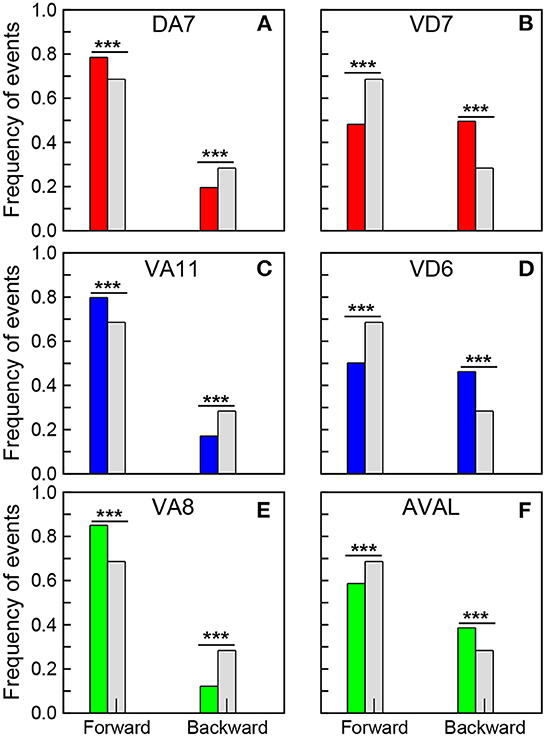
\includegraphics[width=\imsize]{neuronas_comportamiento.jpg}
	\caption[ Correlación de la dinámica neuronal con las acciones del robot.]{Correlación de la dinámica neuronal con las acciones del robot. Fracción de eventos de avance y retroceso registrados cuando las neuronas seleccionadas dispararon. (A) DA7, (C) VA11 y (E) VA8 corresponden a las neuronas con el mayor PC1 positivo en los grupos sincronizados $\Omega_1, \Omega_2$ y $\Omega_3$, mientras que (B) VD7, (D) VD6 y (F) AVAL corresponden a las neuronas con el PC1 negativo más bajo en estos grupos. Las barras grises corresponden a la fracción de eventos de avance y retroceso en un experimento de 20 minutos de duración. Una prueba de chi-cuadrado (estadísticamente significativa, $***p-value < 0.00001$) muestra que los efectos opuestos de todas estas neuronas en las acciones del robot son significativos.}\label{fig:neuronas_comportamiento}
\end{figure}


\begin{table}[h!]
	\centering
	\caption[Fracción de eventos hacia adelante y hacia atrás registrados cuando las neuronas correspondientes se dispararon.  ]{ Fracción de eventos hacia adelante y hacia atrás registrados cuando las neuronas correspondientes se dispararon.   La fracción de eventos para todo el experimento de 20 minutos fue Adelante = 0.69 y Atrás = 0.28.}
	\begin{tblr}{colspec={lll},
			row{odd} = {bg=gray8},
			row{even} = {bg=gray9},
			row{1} = {bg=red3, fg=white, font=\sffamily},
		}
		
Neurona & 	Adelante &	Atrás\\
DA7 &	0.79 &	0.20\\
VD7	& 0.48 &	0.50\\
VA11 &	0.80 &	0.17\\
VD6	& 0.50&	0.46\\
VA8	& 0.85 &	0.12\\
AVAL&	0.59&	0.39
		
	\end{tblr}
	\label{table:neuronas_comportamiento}
\end{table}

\subsection{Discusión}

Sorprendentemente, también observamos la emergencia de una estructura jerárquica anidada. En el gusano, Kaplan et al. \cite{kaplan_nested_2020} mostraron que la presencia de una estructura jerárquica en la dinámica neural permite la coordinación de comportamientos a través de diferentes escalas de tiempo. Esto incluye los movimientos de la cabeza, las ondulaciones del cuerpo y también los episodios de avance y retroceso. Vale la pena recalcar que el diseño simple del robot que utilizamos no permite la ejecución de algunos de estos comportamientos. Sin embargo, Kaplan et al. \cite{kaplan_nested_2020} observaron que la estructura jerárquica persistía incluso cuando los animales estaban inmovilizados, concluyendo que es una propiedad intrínseca que emerge de las neuronas y sus interacciones en los circuitos. Los resultados obtenidos con el robot destacan esta conclusión, es decir, que la presencia de una dinámica anidada es una propiedad emergente de las interacciones de las neuronas a través del conectoma.



\section{Discusión}

El nematodo C. elegans ha sido un organismo modelo de elección en la investigación neurocientífica debido a su capacidad para ofrecer una visión integrada de cómo el sistema nervioso, el cuerpo y el entorno interactúan como un sistema dinámico acoplado. Dos estudios destacados de Kato et al. \cite{kato_global_2015} y Kaplan et al. \cite{kaplan_nested_2020} han demostrado que el comportamiento de C. elegans se encuentra codificado en una jerarquía de dinámicas neuronales de baja dimensión. Estos hallazgos respaldan la hipótesis de que los estados de comportamiento emergen de la interacción neuronal y de circuitos complejos.

En este contexto, hemos aplicado un modelo robótico basado en el conectoma de C. elegans para explorar y poner a prueba estas ideas. No buscábamos replicar al gusano exactamente, sino construir robots inspirados en la conceptualización de Busbice. La elección se basó en el diseño simplificado de estos robots, que permite un enfoque de sistema complejo. A través de esta aproximación, hemos observado diversas características emergentes que también se manifiestan en C. elegans, incluyendo la formación de grupos sincronizados de actividad neuronal correlacionados con acciones.

Nuestros experimentos han revelado que el robot a menudo muestra comportamientos coherentes con las observaciones en C. Elegans. Esto sugiere que la integración de un conectoma en una entidad mecánica abre un abanico de oportunidades para futuras investigaciones. A medida que continuamos refinando nuestra capacidad para emular la dinámica neuronal, y para modelar una neurona con mayor precisión dentro de un conectoma completo, la exploración de los sistemas nerviosos se torna más accesible y ética en comparación con la experimentación con animales.

Nuestros hallazgos respaldan la idea de que la estructura de red del conectoma de C. elegans es fundamental para su dinámica neuronal. Estos resultados podrían extenderse a otros conectomas, ya que hemos identificado principios comunes en la organización de sistemas nerviosos en diferentes especies \cite{heuvel_comparative_2016}. Al mismo tiempo, las diferencias en los resultados pueden proporcionar insights valiosos sobre las adaptaciones específicas de cada especie.

A medida que avanzamos hacia redes neuronales de mayor envergadura y detalle, nos enfrentamos a nuevos desafíos relacionados con la complejidad y la alta dimensionalidad de los datos. El conectoma del hemicerebro de Drosophila, que involucra un gran número de neuronas \cite{scheffer_connectome_2020}, ejemplifica esta complejidad. Nuestro modelo robótico simple, sin embargo, proporciona una herramienta útil para probar hipótesis relacionadas con la estructura y la función del sistema nervioso.

Además, la implementación de conectomas funcionales en robots podría impulsar la investigación en robótica autónoma. Por ejemplo, la capacidad de emular a un organismo en la búsqueda de comida o la detección de sobrevivientes en un edificio derrumbado podría tener aplicaciones en situaciones de desastre. La extensión de este enfoque a otros conectomas de nivel superior, como los de peces, drosófilas y ratones, promete expandir significativamente nuestro conocimiento en neurociencia.

En la segunda parte de nuestra investigación, nos adentramos en el apasionante campo de la hipótesis de criticidad neuronal. Esta hipótesis postula que los organismos están optimizados para operar en el punto crítico, que es un estado intermedio entre el caos y el orden. Similar a las transiciones de fase en la física, en este estado, los organismos pueden realizar comportamientos complejos y adaptarse a su entorno de manera eficiente. Hasta el momento, la literatura científica carecía de estudios que investigaran si un organismo tan pequeño como C. elegans muestra signos de comportamientos complejos relacionados con la criticidad neuronal.

La próxima fase de nuestra tesis busca abordar esta pregunta fundamental: ¿Existen indicios de criticidad neuronal en C. elegans? Para responder a esta pregunta, realizaremos un análisis detallado utilizando datos experimentales de C. elegans reales y un modelo basado en el trabajo de Haimovici et al. Estos esfuerzos llenarán un vacío en la investigación y arrojarán luz sobre si C. elegans opera en un estado de criticidad neuronal, lo que tendría implicaciones significativas para nuestra comprensión de la biología y la neurociencia.






























